\pagecolor{bg}
\thispagestyle{empty}
\text{}
\vfill
\noindent
\begin{minipage}[t]{0.35\textwidth}
	\begin{flushright}
		\textcolor{goban}{\large
			\\
			三十輻共一轂，\\
			當其無，有車之用。\\
			\vspace{0.5em}
			埏埴以為器，\\
			當其無，有器之用。\\
			\vspace{0.5em}
			鑿戶牖以為室，\\
			當其無，有室之用。\\
			\vspace{0.5em}
			故有之以為利，\\
			無之以為用。}
	\end{flushright}
\end{minipage}%
\hfill
{\color{goban}\vrule}
\hfill
\begin{minipage}[t]{0.55\textwidth}
	\vspace{1pt}
	\raggedright
	\textcolor{goban}{\emph{
			Thirty spokes converge to form a wheel hub.\\
			But it is the emptiness inside the hub that makes it useful.\\
			\vspace{0.8em}
			Clay is kneaded to form a pot.\\
			But it is the emptiness inside it that makes it useful.\\
			\vspace{0.8em}
			Doorways and window bays are chiselled to form a house.\\
			But it is the emptiness inside it that makes it useful.\\
			\vspace{0.8em}
			Substance brings benefits.\\
			Emptiness brings usefulness.}
	}
\end{minipage}

\vspace{1em}
\hfill {\textcolor{goban}{道德經 — \textsc{Dàodé Jīng, Chapter 11}}}


\vfill
\begin{center}
\begin{tikzpicture}[>=stealth]
	% PALETA DE LA PORTADA
	\definecolor{bpbg}{HTML}{0B2450}
	\definecolor{textcolor}{HTML}{efce8f}
	\definecolor{sealred}{HTML}{9E2A2B}
	
	% Fondo opcional (descomentar si la página entera debe ser azul)
	% \fill[bpbg] (current page.south west) rectangle (current page.north east);
	
	% Centro de la composición
	\coordinate (Centro) at (0,0);
	
	% El halo del vacío central (donde "reside su utilidad")
	\draw[textcolor, line width=0.3pt, opacity=0.2] (Centro) circle (1.2cm);
	
	% Los 30 radios del Capítulo 11 del Daode Jing (360 / 30 = 12 grados)
	\foreach \a in {0, 12, ..., 348} {
		
		% El radio exterior: materia continua (Parte I)
		\draw[textcolor, line width=0.4pt, opacity=0.75]
		(\a:4.0cm) -- (\a:1.6cm);
		
		% Discretización hacia el vacío: coordenadas matemáticas (Parte II)
		\foreach \r/\op in {1.45/0.8, 1.35/0.5, 1.25/0.25} {
			\fill[textcolor, opacity=\op] (\a:\r cm) circle (0.6pt);
		}
	}
	
	% El Sello de la vacuidad / Estado e=0
	\node[
	fill=sealred,
	draw=textcolor,
	line width=0.4pt,
	inner sep=3.5pt,
	rounded corners=1pt,
	font=\fontsize{14}{14}\selectfont,
	text=textcolor,
	text opacity=0.95
	] at (Centro) {無};
	
\end{tikzpicture}
\end{center}

\vfill
\newpage
\pagecolor{white}

{\centering\chapter{Foundation}\label{parte2}}
\thispagestyle{empty}
\section{Go in two dimensions and two players}

\begin{wrapfigure}[12]{r}{0.33\textwidth}
	\centering
	\vspace{-10pt}
	\begin{goban}[hoshi=false]
		\mark[filled square, fill = {true, color = bg}]{E5}
		\marks[filled circle, fill = {true, color = Moss}]{D5, F5, E4, E6}
	\end{goban}
	\caption{Point $(5,5)$ in \textcolor{bg}{blue}, adjacencies in \textcolor{Moss}{green}.}
	\label{fig:Fig 13}
\end{wrapfigure}
Let us interpret the board in a convenient manner by considering just its points of intersection. Let $n, m \in \mathbb{N}$. We define $N = \{1, \dots, n\}$ and $M = \{1, \dots, m\}$. With these sets, we formalize the game space:\footnote{We use the letter $G$ because we will adopt Japanese Go terminology for our notation whenever it does not lead to confusion. In Japanese, the board is called \textit{Goban} (碁盤).}
$$  G \coloneqq N \times M = \{(x,y) : x \in N,\, y \in M\}.  $$

Let $t_1, t_2 \in G$ be two \textit{points}.\footnote{The letter $t$ originates from the term \textit{ten} (点), meaning point in Japanese (and Chinese).} If $t_1=(a,b)$, we say that $t_2$ is adjacent to $t_1$, denoted by $t_1 \sim t_2$, if it satisfies exactly one of the following conditions:
\begin{align*}
t_2 = (a+1,b), \quad t_2 = (a,b+1),\\
t_2 = (a-1,b), \quad t_2 = (a,b-1).
\end{align*}
If none of these conditions hold, $t_1$ is not adjacent to $t_2$, which we denote by $t_1 \nsim t_2$. Figure~\ref{fig:Fig 13} illustrates the adjacencies of a point.
Having established the \textit{where}, let us examine \textit{who} participates in it. When reviewing the rules, we observed that each point on the board can be in one of three possible states: unoccupied, occupied by a white stone, or occupied by a black stone. We define $E$ as the set of states that a point may assume, $E=\{0,1,2\}$.

These values represent, respectively: vacant, black, and white. With this, we can account for all possible states on the board:
\begin{align*}
	E \times G &= \{(e,t) : e \in E, t \in G \}.
\end{align*}
For example, the point $(4,4) \in G$ may be found in one of three states: $(0,(4,4))$, meaning no stone at $(4,4)$; $(1,(4,4))$, a black stone at $(4,4)$; or $(2,(4,4))$, a white stone at $(4,4)$.

We shall refer to the elements of $E \times G$ as \textit{stones}, denoted by the letter $i$, such that $i=(e,t)$,\footnote{From the term \textit{ishi} (石), meaning ``stone'' in Japanese.} with $e \in E$ and $t \in G$. 

In Go, however, a single point cannot exhibit all states simultaneously; it assumes at most one.

\begin{definition}[Board]
	A subset $T \subseteq E \times G$ is said to be a \textit{board} if,
	$$\forall t \in G, \exists! e \in E \text{ such that } (e, t) \in T.$$

\end{definition}

That is, in $T$ there is a unique state for each position. Having established the \textit{where} and \textit{who}, we can construct the \textit{what}. To do so, we require two fundamental functions:

\begin{definition}[Stone State Function]
	\label{funcioncolor}$$\text{We define } C: E \times G \to E, \quad (e,t) \mapsto e.$$
	\end{definition}
	
\begin{definition}[Stone Position Function]
	\label{funcionposiciion}$$\text{We define } P: E \times G \to G, \quad (e,t) \mapsto t.$$
	\end{definition}
	
Equipped with these, the notion of a group arises naturally:

\begin{definition}[Connection]
	Given a board $T$ and $i_1, i_2 \in T$ two stones. We say that $i_1$ and $i_2$ are connected, denoted by $i_1 \leftrightarrow i_2$, if
	$$C(i_1) = C(i_2) \quad \text{and} \quad P(i_1) \sim P(i_2).$$
\end{definition}

Figure~\ref{fig:def_connection} illustrates the two conditions required for a direct connection $i_1 \leftrightarrow i_2$: the stones must occupy orthogonally adjacent intersections ($P(i_1) \sim P(i_2)$) and share the exact same state ($C(i_1) = C(i_2)$).

\begin{figure}[H]
	\centering
	\begin{goban}[7, hoshi = false,label = {at = {south, west}}]
		% Connected pair: same color and orthogonally adjacent
		\stones[b, mark = {filled circle, fill = {true, color = Moss}}]{B5, C5}
		% Not connected (different states despite P(i_1) ~ P(i_2))
		\stone[b, mark = {filled circle, fill = {true, color = sealred}}]{B2}
		\stone[w, mark = {filled circle, fill = {true, color = sealred}}]{C2}
		% Not connected (same state, but diagonal / non-adjacent positions P(i_1) \not\sim P(i_2))
		\stones[w, mark = {filled circle, fill = {true, color = terracotta}}]{E4, F5}
	\end{goban}
	\caption{Connection between stones. The black stones at $B5$ and $C5$ (\textcolor{Moss}{green}) satisfy $C(i_1) = C(i_2)$ and $P(i_1) \sim P(i_2)$, so they are connected ($i_1 \leftrightarrow i_2$). By contrast, the stones at $B2$ and $C2$ (\textcolor{sealred}{red}) are adjacent in position but differ in state ($C(i_1) \neq C(i_2)$), whereas the white stones at $E4$ and $F5$ (\textcolor{terracotta}{orange})
		share the same state but lie on diagonal intersections ($P(i_1) \not\sim P(i_2)$);
		neither pair is connected.}
	\label{fig:def_connection}
	\end{figure}

\begin{definition}[Group of Stones]
	Let $T$ be a board. Two stones $i_a, i_b \in T$ belong to the same connected component, denoted by $i_a \equiv i_b$, if $i_a = i_b$ or if there exists a finite tuple of stones $(i_1, i_2, \dots, i_k)$ in $T$ ($k \ge 2$) such that
	\[
	i_1 = i_a, \quad i_k = i_b, \quad \text{and} \quad i_m \leftrightarrow i_{m+1} \quad \text{for all } 1 \le m < k.
	\]
	The relation $\equiv$ is an equivalence relation on $T$. Since connected stones share the same state, the state function $C$ extends naturally to each equivalence class $I \in T / {\equiv}$ by setting $C(I) = e$, where $C(i) = e$ for all $i \in I$.
	
	For each state $e \in E$, we define the family of components of state $e$ on $T$ as\footnote{From \emph{ishi} (石, stone/stones). Capitalized to signify sets of stones, and indexed by state $e$ to denote the family of all such components on the board. When the board varies over time, we write $I^e(T)$.}
	\[
	I^e := \{ I \in T / {\equiv} : C(I) = e \}.
	\]
	For $e \neq 0$, the elements $I \in I^e$ are called \emph{groups} of color $e$ (when $|I| = 1$, $I = \{i\}$ corresponds to an \emph{isolated stone}; when $|I| \ge 2$, $I$ is a group). For $e = 0$, the elements $R \in I^0$ are called \emph{regions}.
\end{definition}

Figure~\ref{fig:def_groups_regions} illustrates how the equivalence relation $\equiv$ partitions the board $T$ into groups of stones ($I^1$ and $I^2$) and empty regions ($I^0$).

\begin{figure}[H]
	\centering
	\begin{goban}[7, hoshi = false,label = {at = {south, west}}]
		% Isolated black stone (|I| = 1)
		\stone[b, mark = {filled circle, fill = {true, color = terracotta}}]{B6}
		% Connected black group via a chain of length 4
		\stones[b, mark = {filled circle, fill = {true, color = Moss}}]{B2:D2, D3}
		% Two distinct white groups (diagonal at E5/F4, so not connected)
		\stones[w, mark = {filled circle, fill = {true, color = bg}}]{D5:E5, E6}
		\stones[w, mark = {filled circle, fill = {true, color = amethyst}}]{F3:4, G3}
	\end{goban}
	\quad
	\begin{goban}[7, hoshi = false,label = {at = {south, west}}]
		% Black and white groups enclosing two corner regions
		\stones[b]{A3:C3, C1:2}
		\stones[w]{E7, E5:6, F5, G5}
		% Empty region R_1 in the lower-left corner
		\marks[filled square, fill = {true, color = sealred}, line = {color = black}]{A1:2, B1:2}
		% Empty region R_2 in the upper-right corner
		\marks[filled square, fill = {true, color = teal}, line = {color = black}]{F6:7, G6:7}
	\end{goban}
	\caption{Equivalence classes in $T / {\equiv}$. Left: The family $I^1$ consists of an isolated black stone at $B6$ (\textcolor{terracotta}{orange}) and a four-stone black group (\textcolor{Moss}{green}, where $B2 \equiv D3$ via the chain $B2 \leftrightarrow C2 \leftrightarrow D2 \leftrightarrow D3$), while $I^2$ consists of two distinct white groups (\textcolor{bg}{blue} and \textcolor{amethyst}{purple}). Right: The vacant intersections are partitioned into three regions in $I^0$: the lower-left region $R_1$ (\textcolor{sealred}{red}), the upper-right region $R_2$ (\textcolor{teal}{teal}), and the remaining unmarked vacant region.}
	\label{fig:def_groups_regions}
\end{figure}

From now on, unless explicitly stated otherwise, the letter $I$ will denote a group of non-zero color ($I \in I^e$ with $e \neq 0$), whereas $R$ will denote an empty region ($R \in I^0$).


\begin{definition}[Adjacencies of a Group or Region]
	Let $X \in T / {\equiv}$ be a group or region, and let $i = (e', t) \in T$ be a stone on the board. We say that $X$ is adjacent to $i$, denoted by $X \sim i$, if at least one stone in $X$ is adjacent to $i$:
	\[
	X \sim i \iff \exists i_k \in X : P(i_k) \sim P(i).
	\]
\end{definition}


It will prove very useful to identify the adjacencies of a stone, group, or region.
To this end, we define the set $K$\footnote{From the term \emph{chikaku} (近く, near/nearby).}
associated with them (see Figure~\ref{ejemplo_adyacencias}).
\begin{figure}[H]
	\centering
	\begin{goban}[7, hoshi = false]
		\stones[b]{C5, D5, E4, E5}
		\stones[w]{D3, D4}
		\marks[filled circle, fill = {true, color = Moss}]{B5, C4, C6, D4, D6, E3, E6, F4, F5}
	\end{goban}
	\caption{A black group with its \textcolor{Moss}{adjacencies} (including both vacant intersections and the adjacent white stone at $D4$).}
	\label{ejemplo_adyacencias}
\end{figure}

\begin{definition}[Adjacency Set]\label{def_adjacency}
	Given a board $T$, let $i \in T$ be a stone and let $X \in T / {\equiv}$ be a group or region. We define the adjacency set of the stone $i$ as
	\[
	K(i) = \{ i_r \in T : P(i) \sim P(i_r) \}.
	\]
	For a group or region $X \in T / {\equiv}$, we define
	\[
	K(X) = \{ i \in T \setminus X : X \sim i \}.
	\]
\end{definition}


To characterize the states of these adjacencies, we apply the state function $C$ to the adjacency set.

\begin{definition}[State of the Adjacencies of a Group or Region]
	Given a board $T$, let $X \in I^e$ be a group or region of state $e \in E$. Applying the function $C$ elementwise to its adjacency set $K(X)$, we obtain the set of adjacent states, defined as
	\[
	C(K(X)) := \{ C(i) \mid i \in K(X) \} \subseteq E \setminus \{e\}.
	\]
\end{definition}

This definition is essential for describing much of the internal dynamics of Go.

\begin{definition}[Territory]
	A region $R \in I^0$ is \emph{territory} belonging to the player of color $e \in E \setminus \{0\}$ if $K(R) \neq \emptyset$ and there exists a non-empty family of groups $S \subseteq I^e$ such that
	\[
	K(R) \subseteq \bigcup_{I \in S} I.
	\]
	That is to say, all stones adjacent to the region belong to groups of the same color $e$. We shall denote the territories of each color as\footnote{From the term \textit{ji} (地), meaning ``land'' in Japanese.}
	\[
	J^e := \{ R \in I^0 : C(K(R)) = \{e\} \}, \quad e \neq 0.
	\]
	Regions that do not constitute territory for any player will be denoted and defined as
	\[
	J^0 := \{ R \in I^0 : |C(K(R))| \neq 1 \}.
	\]
\end{definition}
\begin{figure}[H]
	\centering
\begin{goban}[7, hoshi = false]
	\stones[w]{A6, B4:6, C4, D4, E1:3}
	\stones[b]{C6:7, D5, E5, F1:5}
	\marks[filled circle, fill = {true, color = bg}]{A1:5, B1:3, C1:3, D1:3}
	\marks[filled circle, fill = {true, color = Moss}]{D6:7, E6:7, F6:7, G1:7}
	\marks[filled circle, fill = {true, color = terracotta}]{A7, B7, C5, E4}
\end{goban}
	\caption{\textcolor{bg}{White}, \textcolor{Moss}{black}, and \textcolor{terracotta}{neutral} territory.}
	\label{fig:territorios}
\end{figure}
Figure~\ref{fig:territorios} illustrates the different types of territories. With this, on a two-player board we have established a partition of the set of regions $I^0$, since every region belongs to Black's territory, belongs to White's territory, or forms part of neither player's territory:
\[
I^0 = J^0 \cup J^1 \cup J^2.
\]
\label{posicion_espacial}
Additionally, the cardinality of the adjacency set of an individual stone, $|K(i)|$\footnote{This could be interpreted as the degree of a vertex in graph theory.}, proves remarkably useful for determining its spatial placement on the board. Because $|K(i)|$ is bounded by Lemma~\ref{lem:2n}, a straightforward analysis of the number of adjacencies reveals precisely whether the stone is situated in the interior, on an edge, or in a corner.

To formalize captures, we first introduce the concept of a liberty.

\begin{definition}[Liberties of a Group]
	Let $I \in I^e$ be a group of color $e \in E \setminus \{0\}$. We define the set of liberties of said group as
	\[
	L(I) = \{ i \in K(I) : C(i) = 0 \}.
	\]
\end{definition}

Note that if $L(I) = \emptyset$ for a given group, then that group is considered dead. This situation can only occur upon executing a move and effecting a capture. A group is captured when it loses all of its liberties, and captured stones are removed from the board.

\begin{definition}[Capture Criterion]
	Let $I \in I^e$ be a group of color $e \in E \setminus \{0\}$. Then,
	\[
	I \text{ is captured} \iff L(I) = \emptyset.
	\]
\end{definition}

We favor the phrasing \textit{is captured}, since death is the consequence of a capture.

\section{Toward Movement}

Thus far, we have described the static structure of the board. To model a game, we must incorporate the temporal evolution of play. To this end, we first define the space of all possible moves, which we denote by $\mathcal{J}$:
$$\mathcal{J} \coloneqq \left((E \setminus \{0\}) \times G\right) \cup \{\varnothing\}.$$

\subsection{Move Function and Legality}\label{criterio_jugada}
When playing Go on our turn, we either take a stone and place it on the board, or else we pass. We define the move function as $f: \mathbb{N} \to \mathcal{J}$. Let us examine an example. (See Figure~\ref{fig_ej_mov})
\begin{align*}
f(1) &= (1,(2,2)), & f(2) &= (2,(5,4)), & f(3) &= (1,(2,3)),\\
f(4) &= (2,(4,4)), & f(5) &= (1,(3,3)), & f(6) &= (2,(3,2)),\\
f(7) &= (1,(4,5)), & f(8) &= (2,(4,3)), & f(9) &= (1,(3,5)),\\
f(10) &= (2,(2,1)), & f(11) &= \varnothing, & f(12) &= \varnothing.
\end{align*}
\begin{figure}[H]
	\centering
\begin{goban}[7, hoshi = false]
	\moves{B2, E4 ,B3, D4, C3, C2, D5, D3, C5, B1}
\end{goban}
\caption{Reconstructed game on a board.}
\label{fig_ej_mov}
\end{figure}
The function records the moves, but not their legality. Let us analyze the rules. The \textit{suicide rule} prohibits placing a stone if doing so results in the immediate capture of one's own group (Figure~\ref{sui_ej}). There exists a single exception: a move played with no liberties is legal if it simultaneously captures a group of the opposite color (see Figure~\ref{fig: fig1.19}). Note that, due to this mechanic, when it is Black's turn, only white groups may be captured, and vice versa.
\begin{figure}[H]
	%\begin{figure}[H]
	\centering
\begin{goban}[7]
	\stones[b]{D3:4, E3, E5, F3, F5, G4}
	\stone[w]{F4}
	\mark[filled square, fill = {true, color = BlueViolet}, line = {color = black}]{E4}
\end{goban}
\quad
\begin{goban}[7]
	\stones[w]{D3:4, E3, E5, F3, F5, G4}
	\stone[b]{F4}
	\mark[filled square, fill = {true, color = BlueViolet}, line = {color = black}]{E4}
\end{goban}
	\caption{Left: White plays. Right: Black plays. In \textcolor{BlueViolet}{purple}, illegal moves, as they lead to suicide.}
	\label{sui_ej}
\end{figure}

To evaluate a move, we first verify whether it results in a capture. If so, the move is legal. If it does not capture, we inspect its liberties: if it has none, it constitutes suicide and is therefore illegal; otherwise, it is legal. As noted in Section~\ref{primerreglako}, we must keep the \textit{ko rule} in mind. This rule forbids the immediate recapture of a single stone if doing so reverts the board state precisely to the position of the preceding turn (see Figure~\ref{regla_ko_ej}). 
\begin{figure}[H]
	\centering
\begin{goban}[7, hoshi = false, name = ko1]
	\stones[w]{C4, D5, E4}
	\stones[b]{C3, D2, E3}
	\moves[w]{D3}
\end{goban}
\quad
\begin{goban}[7, hoshi = false, resume = ko1, captures]
	\moves{D4}
\end{goban}
	\caption{Position of a stone under apparent suicide that is legal because it captures.}
	\label{fig: fig1.19}
\end{figure}


\begin{figure}[H]
	\centering
\begin{goban}[7, hoshi = false, resume = {ko1, numbers}]
\end{goban}
\quad
\begin{goban}[7, hoshi = false, resume = ko1, captures]
	\moves{D4}
	\mark[filled circle, fill = {true, color = Moss}]{D3}
\end{goban}
	\caption{White cannot play at the \textcolor{Moss}{green intersection}, as doing so repeats a prior board position.}
	\label{regla_ko_ej}
\end{figure}

The basic \textit{ko rule} is insufficient, as cycles exist where the board position is repeated without immediately recapturing the same stone. See Figure~\ref{ciclo_ko}, in which an earlier position is reached once again via a sequence of captures that do not violate the basic \textit{ko rule}.
\begin{figure}[H]
	\centering
	\begin{goban}[7, hoshi = false, name = borde0]
		\stones[w]{A4, A6, B4:5, C5:6, D6:7}
		\stones[b]{A3, B3, B6:7, C3:4, D5, E3, E5:7}
	\end{goban}
	\quad
	\begin{goban}[7, hoshi = false, resume = borde0,name=borde1]
		\moves[w]{A7}
	\end{goban}
	\quad
	\begin{goban}[7, hoshi = false, resume = borde1,name=borde2]
		\moves[b]{A5}
	\end{goban}
	\quad
	\begin{goban}[7, hoshi = false, resume = borde2]
		\moves[w]{A6}
	\end{goban}
	\caption{Board configuration featuring a three-move cycle.}
	\label{ciclo_ko}
\end{figure}
Because repeating positions is prohibited, we require a more general rule. To illustrate an extreme case, see Figure~\ref{ciclo_inf}.\footnote{There exist examples involving far longer cycles; to explore them in greater depth, see \cite{cicloinfinito}.}
\begin{figure}[H]
	\centering
	\begin{pgfgolayout}[columns = 5]
		\begin{goban}[3, name = t3x3]
			\stones[w]{A1, A3, B2}
			\stones[b]{B1, B3, C2}
		\end{goban}
		\begin{goban}[3, name = t3x3-1, resume = t3x3]
			\moves[w]{C3}
		\end{goban}
		\begin{goban}[3, name = t3x3-2, resume = {t3x3-1}]
			\moves{A2}
		\end{goban}
		\begin{goban}[3, name = t3x3-3, resume = {t3x3-2}]
			\moves{C1}
		\end{goban}
		\begin{goban}[3, name = t3x3-4, resume = {t3x3-3}]
			\moves{B3}
		\end{goban}
		\begin{goban}[3, name = t3x3-5, resume = {t3x3-4}]
			\moves{A1}
		\end{goban}
		\begin{goban}[3, name = t3x3-6, resume = t3x3-5]
			\moves{C2}
		\end{goban}
		\begin{goban}[3, name = t3x3-7, resume = t3x3-6]
			\moves{A3}
		\end{goban}
		\begin{goban}[3, name = t3x3-8, resume = t3x3-7]
			\stones[w]{A1, A3, B2}
			\stones[b]{B1, B3}
			\moves{C2, from =8}
		\end{goban}
	\end{pgfgolayout}
	\caption{A cycle of length 8 (assuming external group connections that leave the captured stones with their last liberty inside the $3\times 3$ sub-region) that can be repeated indefinitely in the absence of a Superko rule.}
	\label{ciclo_inf}
\end{figure}
One might argue that on the board in Figure~\ref{ciclo_ko}, the position has indeed repeated, but the turn belongs to the other player; hence, it is not a full repetition. This line of reasoning leads to what is known as the \textit{Natural Superko} rule. We, however, shall adopt a more restrictive variant:
\begin{definition}[Positional Superko]\label{sec-superko}
	A player may not place a stone in such a way that it recreates a board position that has already appeared previously in the game.
\end{definition}
By this rule, in both Figure~\ref{ciclo_ko} and Figure~\ref{ciclo_inf}, any attempt to repeat a cycle will require intermediate moves that generate genuine game progress.

It remains to consider the most elementary restriction in Go: it is not permitted to play on an intersection that is already occupied by another stone.

\begin{definition}[Vacant State Condition]
	Let $T_{n-1}$ be the board prior to turn $n$. For a candidate move $f(n) =(e, p)$ to be playable at turn $n$, the corresponding point $p$ must previously be unoccupied in $T_{n-1}$. This is expressed as:
	$$f(n) = (e, p) \text{ is playable on } T_{n-1} \iff (0, p) \in T_{n-1}.$$
	\end{definition}

Having established the \textit{where}, \textit{who}, and \textit{what}, let us examine the \textit{how}.

\subsection{Legal Move Theorem}

We have seen that a candidate stone $i = (e, p)$ is playable on $T_{n-1}$ if $(0, p) \in T_{n-1}$.
Let $T' = (T_{n-1} \setminus \{(0, p)\}) \cup \{i\}$ denote the tentative board obtained by placing $i$, and let $I(i) \in I^e(T')$ be the unique group of color $e$ containing $i$ on $T'$.

A move is non-suicidal if $L_{T'}(I(i)) \neq \emptyset$.

To detect a capture, we inspect $T'$ to verify whether there exists any adjacent opposing group $X \in I^{e'}(T')$ (with $e' \in E \setminus \{0, e\}$) that is thereby left with no liberties. 

This occurs if $L_{T'}(X) = \emptyset$; since the sole liberty remaining to that group was precisely the intersection just played, occupying it effects the capture. Had $L_{T_{n-1}}(X) = \emptyset$ held prior to the move, the group would already have been removed from the board.

Lastly, $f(n) = i$ produces a capture if and only if
\[
\exists e' \in E \setminus \{0, e\}, \; \exists X \in I^{e'}(T') \text{ with } X \cap K_{T'}(i) \neq \emptyset : L_{T'}(X) = \emptyset.
\]

In the case of SuperKo, let $\mathrm{Cap} = \bigcup \{X \in I^{e'}(T') \mid e' \in E \setminus \{0, e\},\, L_{T'}(X) = \emptyset\}$ and $\mathrm{Cap}_0 = \{(0, P(j)) : j \in \mathrm{Cap}\}$, yielding the post-capture board $T'' = (T' \setminus \mathrm{Cap}) \cup \mathrm{Cap}_0$. We define the Boolean functions $\mathrm{Vacant}$, $\mathrm{Suicide}$, $\mathrm{Capture}$, and $\mathrm{SKo}$. These functions take a candidate move $f(n) = i = (e, p)$ as their argument and return $1$ if the condition is satisfied, and $0$ otherwise:
\[
\mathrm{Vacant}(f(n)) = \begin{cases}
	1 & \text{if } (0, p) \in T_{n-1},\\
	0 & \text{if } (0, p) \notin T_{n-1}.
\end{cases}
\qquad
\mathrm{Capture}(f(n)) = \begin{cases}
	1 & \text{if it captures on } T',\\
	0 & \text{otherwise.}
\end{cases}
\]
\[
\mathrm{Suicide}(f(n)) = \begin{cases}
	1 & \text{if } L_{T'}(I(i)) = \emptyset,\\
	0 & \text{if } L_{T'}(I(i)) \neq \emptyset.
\end{cases}
\qquad
\mathrm{SKo}(f(n)) = \begin{cases}
	1 & \text{if } \exists k: T'' = T_k,\\
	0 & \text{otherwise.}
\end{cases}
\]
With these functions, we can formally characterize when a move is legal.

\begin{theorem}[Legal Move Theorem]\label{teo_jugada_legal}
	Let $f(n) = i \in (E \setminus \{0\}) \times G$ be a move at turn $n$ of a Go game. Said move is legal if and only if it satisfies the following logical proposition:
	$$f(n) \text{ is legal} \iff \text{Vacant} \wedge \neg \text{SKo} \wedge (\neg \text{Suicide} \vee \text{Capture}).$$
	\end{theorem}
\begin{proof}
	
	$(\Rightarrow)$ Suppose that $f(n)$ is a legal move.
	By definition, a legal move does not violate the \textit{Superko} rule; hence $\text{SKo}(f(n))=0$, and consequently $\neg\text{SKo}(f(n))=1$.
	Furthermore, we know that the \textit{suicide rule} prohibits suicidal moves unless they result in a capture. That is, either the move is not a suicide, or (if it is) it necessarily effects a capture. In logical terms, since $f(n)$ is legal, the proposition $\neg\text{Suicide} \vee \text{Capture}$ is always true.
	
	The move must be placed on a vacant point on the board; that is, $\text{Vacant}(f(n))=1$.
	
	
	There exist only three categories of legal moves:
	\begin{enumerate}
		\item The intersection is vacant, there is no \textit{Superko}, there is no suicide, and no stones are captured.
		\item The intersection is vacant, there is no \textit{Superko}, there is no suicide, and a capture occurs.
		\item The intersection is vacant, there is no \textit{Superko}, there is suicide, but a capture occurs.
	\end{enumerate}
	$(\Leftarrow)$ Let us examine the truth table of our proposition. We denote \text{Suicide} by $S$ and \text{Capture} by $\text{Cap}$ for readability. We omit the cases where \textit{Superko} is violated ($\text{SKo}=1$) or where the intersection is occupied ($\text{Vacant}=0$), as they are trivially false.
	\[
	\renewcommand{\arraystretch}{1.2}
	\setlength{\tabcolsep}{10pt}
	\begin{array}{cccccc}
		\toprule
		\text{Vacant} & \neg \text{SKo} & \neg S & \text{Cap} & \neg S \vee \text{Cap} & \text{Vacant} \wedge \neg \text{SKo} \wedge (\neg S \vee \text{Cap}) \\ 
		\midrule
		1 & 1 & 1 & 1 & 1 & 1 \\
		1 & 1 & 1 & 0 & 1 & 1 \\
		1 & 1 & 0 & 1 & 1 & 1 \\
		1 & 1 & 0 & 0 & 0 & 0 \\
		\bottomrule
	\end{array}
	\]
	The truth table demonstrates that the only rows rendering the full proposition true correspond precisely to the three configurations deduced in the forward direction.
\end{proof}

Furthermore, we have characterized not only when a move is legal, but also which types of moves exist:
\begin{enumerate}
	\item Placing a stone without capturing.
	\item Executing a capture.
	\item Executing a capture by means of suicide.
\end{enumerate}

\subsection{Scoring}\label{contarpuntos}
Eventually, by virtue of Superko and mutual agreement, the game concludes. The winner in Go is the player who amasses the greatest number of points. To compute this, it suffices to sum each player's living stones remaining on the board at the end of the game and add their secured territory. In addition, the \textit{komi} is added to White's total.

Let $T$ denote the cleared final board obtained from $T_{\text{end}}$ after removing all
mutually agreed dead stones (replacing each removed stone $i$ with $(0, P(i))$, or
equivalently assuming all dead stones have been captured prior to the terminal passes).
Denoting Black's score by $S(1)$ and White's score by $S(2)$ on $T$, we obtain:
\[
S(1) = \sum_{I \in I^1(T)} |I| + \sum_{R \in J^1(T)} |R|,
\qquad
S(2) = \sum_{I \in I^2(T)} |I| + \sum_{R \in J^2(T)} |R| + \text{komi}.
\]
To determine the winner, it suffices to evaluate the difference: if $S(2) - S(1) > 0$, White wins; if $S(2) - S(1) < 0$, Black wins.

\section{Go in \texorpdfstring{$n$}{n} Dimensions and with \texorpdfstring{$m$}{m} Players}\label{Go_n_m}

If we transition to an $n$-dimensional space, we require $n$ sets to construct the board. As before, for each dimension $i$, given $n_i \in \mathbb{N}$, we define $N_i = \{1, 2, \dots, n_i\}$. The board is then formed by the Cartesian product:
\[ G = N_1 \times N_2 \times \dots \times N_n. \]
For $m$ players, we extend the set of states to $E = \{0, 1, \dots, m\}$, always reserving the value $0$ for vacant intersections.

\begin{definition}[Adjacency Between Points]
	Let $G = N_1 \times N_2 \times \dots \times N_n$ be the game space, and let $t_1, t_2 \in G$ be two points given by $t_1 = (a_1, a_2, \dots, a_n)$ and $t_2 = (b_1, b_2, \dots, b_n)$.
	
	We say that $t_1$ is adjacent to $t_2$, denoted by $t_1 \sim t_2$, if:
	$$\exists! \ i \in \{1, 2, \dots, n\} : \big( \forall r \neq i, \ a_r = b_r \ \land \ a_i = b_i \pm 1 \big).$$
\end{definition}

When reduced to two dimensions, the condition demands one identical coordinate and another differing by exactly 1, naturally recovering the definition of the classical board. Likewise, we extend the notion of connection between stones.

\begin{definition}[Connection]
	Let $T$ be a board and let $i_1, i_2 \in T$ be two stones such that $i_1 = (e, t_1)$ and $i_2 = (e', t_2)$. These are connected if:
	$$i_1 \leftrightarrow i_2 \iff t_1 \sim t_2 \text{ and } C(i_1) = C(i_2).$$
\end{definition}
From now on, whenever we refer to this type of connection, we shall call it \textit{orthogonal adjacency}, since we will see that it is possible to employ other criteria in Part~\ref{parte3}.

The definitions of groups remain identical, as they depend solely on the connection between stones. In turn, territories and captures function in exactly the same manner, since we only require the adjacencies of the group. The only element that truly changes upon introducing more players is the capture criterion; more specifically, the manner in which points are distributed upon removing opposing stones.

Before proceeding, let us highlight a geometric property of vital importance for the subsequent sections.


\begin{lemma}\label{lem:2n}
	On an $n$-dimensional Go board $G = N_1 \times \dots \times N_n$ with $n_i = |N_i| \ge 2$ for all $1 \le i \le n$ and orthogonal adjacency, a point $t=(a_1,a_2,\dots,a_n) \in G$ has at least $n$ and at most $2n$ adjacencies.
\end{lemma}


\begin{proof}
	For each coordinate of $t$, there exists at least one valid direction, since if one is blocked by the edge, the opposite direction remains available (as $n_i \ge 2$). Consequently, each dimension contributes at least one adjacency. At an interior point, each coordinate contributes exactly two. Therefore, there are at least $n$ adjacencies and at most $2n$.
\end{proof}

To simplify notation, we shall adopt the convention of denoting Go in $n$ dimensions and with $m$ players as $\mathrm{Go}^n_m$. Should we wish to explicitly specify the size of each dimension, we may do so in the following manner: $\mathrm{Go}^2_2(19,19)$ for the case of the standard board. If the number of players is omitted, it is to be understood that we are referring to a generic $n$-dimensional board, denoted by $\mathrm{Go}^n$. Likewise, $\mathrm{Go}_m$ will represent a board of arbitrary\footnote{The infinite theory of Go is yet to be developed; I am referring to finite dimension.} dimension played by $m$ players.

\subsection{Captures and Points for \texorpdfstring{$m$}{m} Players}\label{capturas_n_jug}

Let $I$ be a group of stones. Just as on the classical board, for said group to be
considered captured, it must hold that $L(I)=\varnothing$. Consider the $\mathrm{Go}^{2}_{4}$
board illustrated in Figure~\ref{fig:capturasm}. Let us suppose our players are:
blue ($b$), red ($r$), green ($v$), and brown ($t$). Our state set is then defined
as $E = \{0, b, r, v, t\}$.

In this example, we observe that a group of 4 red stones is captured after the brown
player places their stone at position $(6,4)$ ($F4$). However, we note that the red group was not completely surrounded exclusively by terracotta stones. Of the 9 adjacent intersections (the liberties originally possessed by the red group), 3 have been occupied by the green player, 2 by the blue player, and, finally, 4 by the brown player.

How do we distribute the capture points in this scenario? In general, when a group $I$  is captured ($L(I) = \varnothing$), no stone in $K(I)$ has state $0$ or $C(I)$, so the sets $K_c(I) = \{i \in K(I) : C(i) = c\}$ for $c \in E \setminus \{0, C(I)\}$ partition $K(I)$.

Our proposal is to distribute its $|I|$ capture points among each attacking color
$c \in E \setminus \{0, C(I)\}$ in strict proportion to $|K_c(I)|$:
\[\text{Points}_c(I) = \frac{|K_c(I)|}{|K(I)|} \cdot |I|.\]
If the total to be distributed is the 4 points corresponding to the red stones, we allocate
them according to the fraction of adjacencies occupied by each attacker:
\begin{align*}
	\text{Green's points} = \frac{3}{9} \cdot 4,\quad
	\text{Blue's points} = \frac{2}{9} \cdot 4,\quad
	\text{Brown's points} = \frac{4}{9} \cdot 4.
\end{align*}
Indeed, the sum of the parts equals the total number of points:
\[ \left(\frac{3}{9} + \frac{2}{9} + \frac{4}{9}\right) \cdot 4 = 4. \]
\begin{figure}[H]
	\centering
\begin{goban}[7, hoshi = false]
	\stones[fill = {color = sealred}]{C5, D5, E4, E5}
	\stones[fill = {color = terracotta}, line = false]{C4, D4, E3}
	\stones[fill = {color = bg}, line = false]{B5, F5}
	\stones[fill = {color = Moss}, line = false]{C6:E6}
\end{goban}
\quad
\begin{goban}[7, hoshi = false]
	\stones[fill = {color = sealred,opacity=0.28}]{C5, D5, E4, E5}
	\stones[fill = {color = terracotta}, line = false]{C4, D4, E3}
	\stones[fill = {color = bg}, line = false]{B5, F5}
	\stones[fill = {color = Moss}, line = false]{C6:E6}
	\moves[b, from = 1, fill = {color = terracotta}, line = false, label = {color = white}]{F4}
\end{goban}
	\caption{
		Capture in $\mathrm{Go}^{2}_{4}$. Brown plays and captures the red group.}
	\label{fig:capturasm}
\end{figure}
In this manner, a proportional distribution is achieved, rewarding the player who contributes most to the capture. Awarding the points solely to the player who executes the capture would disincentivize aggression; it would be unfeasible to surround an opponent if, during the $m-1$ intermediate turns, others could ``steal'' the capture.
\subsection{Komi for Multiple Players}\label{komi_n_jug}

The origin of \textit{komi} lies in preventing draws and counterbalancing the disadvantage of playing second; therefore, it is necessary to reinterpret this concept when multiple players are involved. What follows is a proposal on how we might generalize it.

\subsection*{Stepped Komi}
We can define \textit{komi} as a function that depends strictly on the turn order. If we consider the set of players $E \setminus \{0\}$, we can establish a compensation constant $\alpha \in \mathbb{Q}$. Thus, the \textit{komi} function $K: E \setminus \{0\} \to \mathbb{R}$ is defined as:
$$K(j) = (j - 1) \cdot \alpha.$$

\subsection*{Irrational Komi}
If we additionally seek to preserve the second historical function of \textit{komi}, preventing draws, we must ensure that no two players can achieve the same score. Let $Q_j \in \mathbb{Q}$ denote the rational score of player $j \in E \setminus \{0\}$ derived from stones, territories, and proportional captures, and let $\gamma_j \in \mathbb{R}$ be the \textit{komi} assigned to player $j$. A tie between players $j$ and $k$ ($j \neq k$) occurs if and only if
$$Q_j + \gamma_j = Q_k + \gamma_k \iff \gamma_j - \gamma_k = Q_k - Q_j \in \mathbb{Q}.$$
Therefore, to guarantee the impossibility of ties, it is necessary and sufficient to assign \textit{komi} values such that $\gamma_j - \gamma_k \notin \mathbb{Q}$ for all $j \neq k$. In particular, choosing an irrational constant $\alpha \in \mathbb{R} \setminus \mathbb{Q}$ in the Stepped Komi formula $\gamma_j = (j - 1)\alpha$ automatically satisfies $\gamma_j - \gamma_k = (j - k)\alpha \notin \mathbb{Q}$ for all $j \neq k$, eliminating any possibility of a tie.

\subsection*{Auction Komi}
Prior to the start of the game, each player $j \in E \setminus \{0\}$ secretly declares a bid $b_j \in \mathbb{Q}$, representing the number of points they are willing to sacrifice from their final score in exchange for the privilege of securing the initiative (i.e., a negative \textit{komi}). Once all bids have been collected, they are revealed. The turn order is established in strictly decreasing order: the player with the highest $b_j$ value will play first, followed by the second highest, and so forth. In the event of a tie between two or more bids, the turn order for those players is resolved in favor of whoever placed their bid first.

These solutions may be employed simultaneously or further refined; what is presented here are ideas on how to rectify the lack of a well-defined \textit{komi} in generalized Go.\footnote{Author's note: In my opinion, \textit{komi} should not exist; the initiative (\textit{sente}) can be lost at any moment. Furthermore, the larger the board, the less it matters who plays first. This 20th-century invention is only useful for professional players.}

\section{Positional Superko Detection}\label{detec_superko}

By virtue of the Legal Move Theorem~\ref{teo_jugada_legal}, which by construction holds for $n$ dimensions, we possess the theoretical tool to determine whether a move is legal; however, thus far we have not discussed the mechanism for its practical detection.

We have already formalized how to determine whether a capture or a suicide occurs, or whether the intended intersection is occupied. Now, when does a \textit{Superko} occur? That is to say, how do we effectively ascertain that we have violated this rule?

A violation of the \textit{Superko} rule implies that the candidate move recreates a board configuration that has already occurred in the game. To detect this, it would suffice to maintain a historical record of the states of every intersection at each turn. Thus, by tentatively simulating the intended move and comparing the resulting state against the history, we could determine that the rule has been broken if an exact match exists.

To solve this problem, we shall make use of the work developed by Albert L. Zobrist~\cite{zobrist1970hashing}.

%		El primer método propone lo siguiente: dado un tablero $\mathrm{Go}^{n}_{m}$, buscamos simplificar la representación espacial de las $n$-tuplas y colapsar todas las coordenadas en un vector. El tamaño o dimensión de este vector será exactamente el cardinal del tablero:
%		\[|T| = \prod_{i=1}^{n} |N_i| = \tau.\]
%		Basta extraer el estado de cada intersección para obtener una $\tau$-tupla que codifica el tablero de manera \textit{ordenada}. Antes de ejecutar una jugada, se simula el tablero resultante y se realiza la siguiente resta con el historial, si convenimos en llamara a este historial $T(t)$, el tablero en el turno $t$, queremos comparar lo siguiente,
%		\[T(t) - T(t-k).\]
%		Para $k = 1, 2, \dots, t-1$. Si el resultado de esta operación es el vector nulo para algún valor de $k$, entonces la posición es idéntica y hemos roto la regla del \textit{SuperKo}. 


%		Veremos que este proceso puede optimizarse considerablemente en términos de la cantidad de comparaciones requeridas.
%		
%		\subsection{Función emparejadora de Cantor}\label{functCantor}
%		
%		Para estos efectos, haremos uso de la función emparejadora de Cantor generalizada (\textit{cpf}).
%		
%		\begin{theorem}
	%			Para todo $n \in \mathbb{N}$, la función emparejadora de $n$-tuplas $\langle \cdot, \dots, \cdot \rangle: \mathbb{N}^{n} \rightarrow \mathbb{N}$, definida como:
	%		\[cpf(X_1, \dots, X_n) = \sum_{h=1}^{n} \left\{ \frac{1}{h!} \prod_{j=0}^{h-1} \left[ \left( \sum_{i=1}^{h} X_i \right) + j \right] \right\}, \quad \forall(X_{1}, \dots, X_{n}) \in \mathbb{N}^{n}.\]
	%			es un polinomio de grado $n$ con coeficientes racionales. Más aún, es una biyección de $\mathbb{N}^n \rightarrow \mathbb{N}$.\footnote{Para ver la demostración, diríjase a \cite{Lisi2007}.}
	%		\end{theorem}
%		
%		Por el teorema, todo tablero puede ser llevado a $\mathbb{N}$. Al ser nuestros tableros finitos, aplicar el teorema produce en una inyección de $G$ en $\mathbb{N}$. Si nuestro tablero $T$ es un subconjunto de $E \times G$, con $E = \{0, 1, 2, \dots, m\}$ y $G = N_1 \times \dots \times N_n$, definiendo el número total de intersecciones como $\pi = |G| = \prod_{i=1}^{n} |N_i|$, obtenemos la siguiente correspondencia:
%		\[ T \leftrightarrow E \times \mathbb{N}_{\pi} = \{(e_1, k_1), (e_2, k_2), \dots, (e_{\pi}, k_\pi)\} \]
%		donde $e_i \in E$ es algún estado y $k_j$ es un número natural único dado por la función. Cabe aclarar que aquí $\mathbb{N}_{\pi}$ no representa el conjunto de los naturales «hasta el número $\pi$», sino un subconjunto específico de números naturales de cardinalidad $\pi$.
%		
%		Con esto, logramos ordenar el tablero: basta con seguir el orden natural de $\mathbb{N}$ en la segunda coordenada. Como lo único que nos importa para la detección de la regla son los estados del tablero (y no los números en sí, podemos dar un paso más. Si aplicamos la función de estado $C$ que definimos en la Sección~\ref{funcioncolor}, obtenemos un vector de dimensión $\pi$:
%		\[ C \circ \textit{cpf} (E \times \mathbb{N}_{\pi}) = (e_{1}, e_{2}, \dots, e_{\pi}) = E^{\pi}. \]
%		Valiéndonos de la biyección, este vector está perfectamente definido, pues a cada piedra $i=(e,t)$ le corresponde un único par $(e, \textit{cpf}(t))$. Esta correspondencia se ilustra en el diagrama conmutativo de la Figura~\ref{diagramacantor}.
%		
%		\begin{figure}[H]
	%			\centering
	%			\[
	%			\begin{tikzcd}
		%				{E \times G} && {E \times \mathbb{N}_{\pi}} \\
		%				\\
		%				{E^{\pi}}
		%				\arrow["\textit{cpf}", leftrightarrow, from=1-1, to=1-3]
		%				\arrow["C"', from=1-1, to=3-1]
		%				\arrow["{C \circ \textit{cpf}}", from=1-3, to=3-1]
		%			\end{tikzcd}
	%			\]
	%			\caption{Diagrama de la composición.}
	%			\label{diagramacantor}
	%		\end{figure}
%		
%		Como el tablero posee un ordenamiento estricto y la función es biyectiva, dos tableros idénticos siempre generarán el mismo vector $E^{\pi}$.
%		
%		Si guardamos el vector $E^{\pi}(t)$ en cada turno $t$, para verificar la legalidad de la jugada actual basta restar $E^{\pi}(t) - E^{\pi}(t-k)$ para todo $k = 1, 2, \dots, t-1$. Si para algún $k$ dicha resta da como resultado el vector nulo ($\vec{0}$), significa que la posición exacta se ha repetido, rompiendo la regla. Formalmente:
%		\[ \text{SuperKo en el turno } t \iff \exists k : E^{\pi}(t) - E^{\pi}(t-k) = \vec{0}. \]
%		Como hemos adelantado, no hace falta realizar las $t-1$ comparaciones. Para que un tablero pueda siquiera tener la posibilidad de ser igual a otro, es una condición necesaria que la cantidad de piedras de cada color sea idéntica en ambos turnos. Es decir, solo computaremos $E^{\pi}(t) - E^{\pi}(t-k)$ si se cumple que, para cada estado $e \in E \setminus \{0\}$:
%		\[ \sum_{I} |I^{e}|_t = \sum_{I} |I^{e}|_{t-k}. \]
%		
%		Podría parecer que estamos realizando cálculos de más, pero el tamaño del tablero ($\pi$) siempre será inmensamente mayor que la cantidad de jugadores ($m$). Guardar el conteo de las piedras exige almacenar solo $m$ números adicionales por turno. Realizar a lo sumo $m$ comparaciones numéricas simples nos permite descartar rápidamente un tablero que, de otro modo, exigiría $\pi$ comparaciones componente a componente. A modo de ejemplo, en el $\mathrm{Go}^{2}_{2}(19,19)$, basta hacer 2 comparaciones preliminares (conteo de blancas y negras) para descartar el análisis de un tablero de $19 \cdot 19 = 361$ puntos. Por lo tanto, nos ahorramos hasta 359 operaciones por turno descartado.
%Veamos un ejemplo con el tablero tradicional. Si tenemos $E\times G$, $E=\{a,e_1,e_2\}$, $G=N\times N$ con $|N|=3$, la función de cantor para 2 dimensiones nos queda:

%$$\langle a,b \rangle =  \sum_{h=1}^{2}\left\lbrace \frac{1}{h!} \prod_{j=0}^{h-1} \left[\ \left( \sum_{i=1}^{h} X_i \right)+j \right]  \right\rbrace=\frac{(a+b)²+3a+b}{2}$$

%Con lo cual, obtenemos la siguiente tabla que corresponde a los puntos evaluados en la función.

%\begin{table}
%	\centering
%		\begin{tabular}{|l|l|ll}
	%			\hline
	%			cdf(x,y) & Número & \multicolumn{1}{l|}{cdf(x,y)}&
	%\multicolumn{1}{l|}{Número} \\ \hline
	%			1,1   & 4      & \multicolumn{1}{l|}{2,3}      & \multicolumn{1}{l|}{18}     \\ \hline
	%			1,2      & 8      & \multicolumn{1}{l|}{3,1}      & \multicolumn{1}{l|}{11}     \\ \hline
	%			1,3      & 13     & \multicolumn{1}{l|}{3,2}      & \multicolumn{1}{l|}{17}     \\ \hline
	%			2,1      & 7      & \multicolumn{1}{l|}{3,3}      & \multicolumn{1}{l|}{24}     \\ \hline
	%			2,2      & 12     &                               &                             \\ \cline{1-2}
	%		\end{tabular}
%	\end{table}

% Obtenemos para cada turno el conjunto (ordenado)
%\begin{align*}
%	E\times M(t)=\{(e_{1},4),(e_{2},7),(e_{3},8),(e_{4},11),(e_{5},12)\\,(e_{6},13),(e_{7},17),(e_{8},18),(e_{9},24)\}.
%\end{align*}

%Con $e_i\in E$, Que podemos simplificar a $E(t)=(e_{1},\dots,e_{9}).$ Entiéndase que los $e_i$ no están dados por el orden, sino que están numerados para mejor legibilidad.
% Que corresponde al tablero dado por

% \begin{align*}
%	E\times G=\{(e_{i_{1}},(1,1)),(e_{i_{2}},(2,1)),(e_{i_{3}},(1,2)),(e_{i_{4}},(3,1)),\\
%	(e_{i_{5}},(2,2)),(e_{i_{6}},(1,3)),(e_{i_{7}},(3,2)),(e_{i_{8}},(2,3)),(e_{i_{9}},(3,3))\}
%\end{align*}

%	  Si bien utilizar \textit{cpf} nos proporciona una biyección y, por lo tanto, una representación infalible para nuestros fines, resulta computacionalmente muy costoso. Evaluar el polinomio para cada posición en tableros masivos y realizar múltiples comparaciones vectoriales en partidas largas es ineficiente.

%	  Afortunadamente, existe otra forma de hacer todo esto en tiempo constante ($O(1)$), con el único inconveniente de que renuncia a la biyección absoluta y adquiere una naturaleza probabilística (puede fallar por colisiones). 


\subsection{Zobrist Hashing}\label{ZobristHash}

For this method, we shall make use of the logical \textit{exclusive or} operator, denoted as XOR ($\oplus$), applied to random numbers $r_i$ represented as $n$-bit integers.

An $n$-bit integer is a sequence of $n$ binary digits. For example, the number 15 in 4 bits is represented as $1111$, since:
\[ 2^3 \cdot 1 + 2^2 \cdot 1 + 2^1 \cdot 1 + 2^0 \cdot 1 = 8 + 4 + 2 + 1 = 15. \]
Likewise, the number 9 in 4 bits is $1001$. Let us recall the truth table for the logical XOR operator (see Figure~\ref{TablaXOR}).
\vspace{10pt}

\begin{wrapfigure}[8]{l}{0.19\textwidth}
	\vspace{-30pt}
	\centering
	\[
	\begin{array}{c|c|c}
		A & B & A \oplus B \\
		\hline
		0 & 0 & 0 \\
		0 & 1 & 1 \\
		1 & 0 & 1 \\
		1 & 1 & 0
	\end{array}
	\]
	\caption{XOR table.}
	\label{TablaXOR}
\end{wrapfigure}\noindent Performing the XOR operation between 15 and 9 in base 2 means applying the operator individually to each corresponding bit. It is worth clarifying that, although we write the numbers contiguously, we actually treat them as if they were, in this case, 4-tuples: $1111 \oplus 1001 = 0110$. If $r_i$ and $r_j$ are independent, uniformly distributed random sequences of $n$-bit integers, the following properties hold:\hfill\break

\begin{enumerate}
	\item[P1)] $( r_i \oplus r_j ) \oplus r_k = r_i \oplus ( r_j \oplus r_k )$. \hfill(Associativity)
	\item[P2)] $r_i \oplus r_j = r_j \oplus r_i$.\hfill (Commutativity)
	\item[P3)] $r_i \oplus r_i = \vec{0}$.\hfill (Nilpotence)
	\item[P4)] If $s = r_1 \oplus r_2 \oplus \dots \oplus r_k$, then $s$ is also a random sequence.
	\item[P5)] The resulting values $s$ are uniformly distributed.
\end{enumerate}

To begin constructing our algorithm, we must take the set of all possible configurations of a stone on the board, namely, $(E \setminus \{0\}) \times G$.
We exclude $0$ since we do not place stones of color $0$ during play. Next, we assign a unique, random $n$-bit integer to each element. If we recall that a player has the option to \textit{pass} their turn (a move that does not alter the board state), this action will be assigned $\vec{0}$, which guarantees that the state remains unchanged (as $\vec{0}$ is the neutral element of the sum).

To initialize the hash table so that all elementary stone-position pairs receive distinct non-zero seeds (plus $\vec{0}$ for the empty board), the minimum bit-length $n$ must satisfy:
\[ 2^n \geq |(E \setminus \{0\}) \times G| + 1. \]
For our case, on the standard board, we will have $361$ intersections and $2$ possible states for the stones (white and black). 
Therefore:
$$|(E\setminus\{0\}) \times G| = 2 \times 361 = 722.$$
Hence, the minimum number of bits required to assign distinct seeds to the basic board table will be $n = 10$, since
$$2^{10} = 1024 \geq 722 + 1.$$

Zobrist warns of the existence of two types of errors. A \textit{Type 1 error} occurs when two distinct board configurations produce exactly the same hash value; in the context of \textit{Superko}, this would result in a false positive. On the other hand, a \textit{Type 2 error} occurs due to memory space limitations, which we shall not consider.
To reduce the probability of a Type 1 error, Zobrist proposes two complementary solutions. The first consists of generating a second hash simultaneously, utilizing an independent sequence, to rule out false positives. The second solution entails using a greater number of bits than strictly necessary. If $N = 2^n$ is the number of stored states we compare against and $m$ is the number of extra bits added (so the hash length is $b = n + m$), Zobrist demonstrates that the probability of a new state avoiding a Type 1 error against $2^n$ states is given by the following expression (see Table~\ref{Tabla_prob}):
$$p(\text{no error}) = \left( 1 - \frac{1}{2^{n+m}} \right)^{2^n} \approx \left( \frac{1}{e} \right)^{2^{-m}},$$
%while across a game of $T$ turns using $b = n + m$ bits, the probability of experiencing zero hash collisions among all $\binom{T}{2}$ pairs of visited states is given by the birthday bound $\prod_{k=1}^{T-1}(1 - k/2^b) \approx \exp(-T(T-1)/2^{b+1})$.
\begin{table}[H]
	\centering
	\begin{tabular}{c|c || c|c}
		\textbf{$m$ (extra bits)} & \textbf{Prob. of no error} & \textbf{$m$ (extra bits)} & \textbf{Prob. of no error} \\ \hline
		0 & 0.36778 & 6  & 0.98449 \\
		1 & 0.60653 & 7  & 0.99222 \\
		2 & 0.77879 & 8  & 0.99611 \\
		3 & 0.88251 & 9  & 0.99805 \\
		4 & 0.93941 & 10 & 0.99901 \\
		5 & 0.96924 & \multicolumn{2}{c}{}
	\end{tabular}
	\caption{Probability of no error by using more bits.}
	\label{Tabla_prob}
\end{table}
Therefore, against $2^{10}$ states, utilizing 21-bit ($m=11$) or 32-bit ($m=22$) numbers achieves a probability of avoiding a Type 1 error of $0.9995$ or $0.99999976$, respectively.

\begin{definition}[SuperKo detection]
	Given a game trajectory $\{T_0, T_1, \dots, T_{t-1}\}$, a play $f(t)\neq \varnothing$ breaks the SuperKo rule exactly when:
	$$\text{SuperKo}(f(t)) = 1 \iff \exists k \in \{1, \dots, t\} : T_t = T_{t-k}.$$
\end{definition}
In the context of Zobrist, to verify the \textit{Superko} rule, it suffices to perform at most $S \cdot t$ operations, where $S$ is the total number of independent hash sequences implemented. If $H_{s}(t)$ represents the hash value at turn $t$ for sequence $s$, then a stone placement $f(t) \neq \varnothing$ triggers a SuperKo detection when:
\[
SuperKo(f(t)) = 1 \Rightarrow \exists k \in \{1, 2, \dots, t\}\ \forall s \in \{1, \dots, S\} :
H_s(t) \oplus H_s(t-k) = \vec{0}.
\]

Furthermore, to process captures, we shall make use of the XOR operator properties assumed previously. When a stone is captured, it is removed from the board. Therefore, if stone $i_{j}$ is removed, it suffices to apply the operation $H_s(t) \oplus h_s(i_{j})$ to the current state.

By virtue of Properties P1 and P2, we can rearrange the hash calculation:
\begin{align*}
	H_s(t) \oplus h_s(i_{j}) &= \big( h_s(i_{1}) \oplus \dots \oplus h_s(i_{j}) \oplus \dots \oplus h_s(i_{m}) \big) \ \textcolor{sealred}{\oplus \ h_s(i_{j})} \\
	H_s(t) \oplus h_s(i_{j}) &= h_s(i_{1}) \oplus \dots \oplus \big( h_s(i_{j}) \ \textcolor{sealred}{\oplus \ h_s(i_{j})} \big) \oplus \dots \oplus h_s(i_{m}) & \text{(P1 and P2)} \\
	H_s(t) \oplus h_s(i_{j}) &= h_s(i_{1}) \oplus \dots \oplus \textcolor{sealred}{\vec{0}} \oplus \dots \oplus h_s(i_{m}). & \text{(P3)}
\end{align*}

Given that the null vector $\vec{0}$ is the identity element of the operation $(\vec{0}\oplus h(i_{p})=h(i_{p}))$, the term vanishes. Thus, we have demonstrated that removing a stone (capturing) is equivalent to adding its hash once again. To conclude this chapter, let us illustrate with a concrete example on a small $\mathrm{Go}^{2}_{2}(3,3)$ board.

Since the board possesses 9 intersections, we have $|(E\setminus\{0\}) \times G| = 18$. Hence, the minimum number of bits $n$ required will be 5, because $2^5 = 32 \geq 18 + 1$. If we decide to append 3 additional bits as a safety margin, we will have 8-bit numbers. To initialize, it suffices to randomly assign a number to each possible state at every intersection. To this end, we construct the following table:
\begin{table}[H]
	\centering
	\small
	\begin{tabular}{lc|lc|lc}
		\textbf{Stone} & \textbf{Number} & \textbf{Stone} & \textbf{Number} & \textbf{Stone} & \textbf{Number} \\ \hline
		(1,(1,1)) & 01111111 & (1,(2,1)) & 00010110 & (1,(3,1)) & 01001101 \\
		(1,(1,2)) & 10001101 & (1,(2,2)) & 11110001 & (1,(3,2)) & 11101111 \\
		(1,(1,3)) & 10111110 & (1,(2,3)) & 10110001 & (1,(3,3)) & 00011110 \\
		(2,(1,1)) & 00001110 & (2,(2,1)) & 00000010 & (2,(3,1)) & 01001110 \\
		(2,(1,2)) & 10010011 & (2,(2,2)) & 10111010 & (2,(3,2)) & 01000111 \\
		(2,(1,3)) & 10110111 & (2,(2,3)) & 10010001 & (2,(3,3)) & 11001100 \\
	\end{tabular}
	\caption{Hash table of each point in the $3\times 3$ board.}
	\label{tablahash}
\end{table}

We initialize the game hash to the null vector $\vec{0} = 00000000 $, representing the empty board. From this point onward, for every executed move, we update the state by applying the XOR operation ($\oplus$) between the hash of the current turn and the value of the newly placed stone (or removed stone, in the event of a capture). Let us suppose that the following sequence of moves is executed, yielding the board shown in Figure~\ref{fig:tablero_ejsko}:
 \begin{align*}
	f(1)&=(1,(2,2)), &f(2)&=(2,(1,3)),	&f(3)&=(1,(2,3)), &f(4)&=(2,(2,1)),\\
	f(5)&=(1,(3,1)), &f(6)&=(2,(3,2)), &f(7)&=(1,(1,2)), &f(8)&=\varnothing,\\
	f(9)&=\varnothing. 
\end{align*} 
%\begin{wrapfigure}[4]{r}{0.5\textwidth}
\begin{figure}[H]
	\centering
	\begin{goban}[3]
		\moves[b, from = 1]{B2, A3, B3, B1}
		\moves[b, from = 5]{C1}
	\end{goban}
	\quad
	\begin{goban}[3]
		\moves[b, from = 1]{B2, A3, B3, B1}
		\moves[w, from = 6]{C2}
	\end{goban}
	\quad
	\begin{goban}[3]
		\moves[b, from = 1]{B2}
		\moves[b, from = 3]{B3, B1}
		\moves[w, from = 6]{C2, A2}
	\end{goban}
	\caption{Finished game on a $3\times 3$ board.}
	\label{fig:tablero_ejsko}
\end{figure}
We shall compute the states turn by turn, partitioning the vectors into 4-bit blocks to facilitate readability. Denoting the hash of a stone by $h(p_i)$, where $p_i = (e, t)$, the evolution of the game proceeds as follows. On the sixth move, a capture is executed upon the black stone at $(3,1)$; consequently, in addition to applying the hash of the newly played stone, we must apply the hash of the removed stone to ``undo'' its presence. Should multiple stones be captured, it would suffice to iterate the operation for each of them in any arbitrary order (by virtue of P1 and P2):
\begin{figure}[H]
	\centering
	\begin{align*}
		H(0) &= \vec{0} \\
		H(1) &= H(0) \oplus \textcolor{bg}{h((1, (2,2)))} = 1111\, 0001 \\
		H(2) &= H(1) \oplus \textcolor{bg}{h((2, (1,3)))} = 0100\, 0110 \\
		H(3) &= H(2) \oplus \textcolor{bg}{h((1, (2,3)))} = 1111\, 0111 \\
		H(4) &= H(3) \oplus \textcolor{bg}{h((2, (2,1)))} = 1111\, 0101 \\
		H(5) &= H(4) \oplus \textcolor{bg}{h((1, (3,1)))} = 1011\, 1000 \\
		H(6) &= H(5) \oplus \textcolor{bg}{h((2, (3,2)))} \oplus \textcolor{sealred}{h((1, (3,1)))} = 1011\, 0010 \\
		H(7) &= H(6) \oplus \textcolor{bg}{h((1, (1,2)))} \oplus \textcolor{sealred}{h((2, (1,3)))} = 1000\, 1000 \\
		H(8) &= H(7) \oplus \textcolor{bg}{0000\, 0000} = H(7) \\
		H(9) &= H(8) \oplus \textcolor{bg}{0000\, 0000} = H(8).
	\end{align*}
	\caption{Game hashes; \textcolor{bg}{moves} in blue, \textcolor{sealred}{captures} in red.}
\end{figure}
At turns 8 and 9, passing the turn produces a state identical to the preceding one. This does not violate the \textit{Superko} rule, as the rule solely prohibits placing a stone to recreate a position.

However, even with all 18 elementary seeds pairwise distinct, it could occur that
$h((2, (3, 2))) = 1011\ 0011 = h((1, (2, 3))) \oplus h((2, (2, 1)))$. This would trigger a false positive for Superko on the sixth turn, since $H(6) = H(5) \oplus h((2, (3, 2))) \oplus h((1, (3, 1))) = 0100\ 0110 = H(2)$ and, upon comparing it with the history, $$H(6) \oplus H(2) = 0000\ 0000.$$
Thus, by employing additional bits and implementing multiple simultaneous sequences to rule out collisions, Zobrist's method is fully implemented in Go.

\section{The Structure of Time}

We are now in a position to inject time into the structure. We define $\mathcal{T}$ as the space of all boards,
$$ \mathcal{T} = \{ T \subseteq E \times G \mid T \text{ is a board}\}.$$

\subsection{The Game as a Trajectory}
A game constitutes a sequence of moves $f : \mathbb{N} \to \mathcal{J}$, where $f(t)$ represents the action chosen by the active player at turn $t$.

This function $f$ naturally induces a sequence of boards in $\mathcal{T}$, which we shall term a trajectory:
$$\{T_0, T_1, \dots, T_{\mathrm{end}}\}$$
The sequence is constructed recursively by means of $\Delta$:

\begin{enumerate}
	\item \textbf{Initial state ($t=0$):} $T_0$ is the empty board; that is, the set $T_0 = \{(0, t) : t \in G\}$.
	\item \textbf{Transition ($t \rightarrow t+1$):} The board at the subsequent turn is the result of applying the transition to the move of the current turn:
	$$T_t = \Delta(T_{t-1}, f(t)).$$
	\end{enumerate}

\subsection{State Dynamics}\label{section_state_dynamic}

Under this construction, we formalize the properties of the game's flow. We shall denote by $E^k(T_t) = \{i \in T_t : C(i) = k\}$ the set of all stones of color $k$ present on the board at turn $t$, and by $|E^k(T_t)|$ its cardinality.

\begin{itemize}
	\item \textbf{Growth and Decrease:} If at turn $t$ the active player is $k \in E \setminus \{0\}$, the new board given by $T_t = \Delta(T_{t-1}, f(t))$ will possess, at most, one additional stone of their color. In contrast, the stones of the other colors ($j \neq k$) can only decrease or remain constant due to potential captures:
	\begin{align*}
		|E^k(T_t)| &\le |E^k(T_{t-1})| + 1,\\
		|E^j(T_t)| &\le |E^j(T_{t-1})|, \quad \forall j \neq k.
	\end{align*}
	
	\item \textbf{Halting Condition:} Let $m = |E \setminus \{0\}|$ be the total number of players. The game concludes at turn $t_{\mathrm{end}} \in \mathbb{N}$ when all players pass consecutively. This occurs when:
	$$f(t_{\mathrm{end}}) = f(t_{\mathrm{end}}-1) = \dots = f(t_{\mathrm{end}}-m+1) = \varnothing.$$
	Consequently, the state of the board freezes, resulting in:
	$$T_{\mathrm{end}} \coloneqq T_{t_{\mathrm{end}}} = T_{t_{\mathrm{end}}-1} = \dots = T_{t_{\mathrm{end}}-m}.$$
	This state $T_{\mathrm{end}}$ constitutes the Final Board.
\end{itemize}

\subsection{Anatomy of a Move}

Let us understand how $\Delta$ functions. Suppose we are playing Go and that, on our turn, we intend to play $f(t)$.
If $f(t) = \varnothing$, the board remains identical and we pass the turn; that is,
$$T_{t} = \Delta(T_{t-1}, \varnothing) = T_{t-1}.$$

If $f(t) = i^{*} = (e, p)$, we must validate said move. The computation of the new board $T_t = \Delta(T_{t-1}, i^{*})$ by virtue of Theorem~\ref{teo_jugada_legal} is performed as follows:
\begin{enumerate}
	\item \textbf{Placement:} If there exists $(e',p)\in T_{t-1}$ such that $e' \neq 0$, the move is illegal. If $e'=0$, we generate a temporary board $T'$ where intersection $p$, previously empty, acquires state $e$. We then proceed to the next step.
	$$T' = \left(T_{t-1} \setminus \{(0, p)\}\right) \cup \{(e, p)\}.$$
	
	\item \textbf{Capture Detection:} Evaluating the adjacencies in $T'$, we identify the set $\mathrm{Cap}$ of all captured stones by taking the union of all opposing groups that possess no liberties:
	\[
	\mathrm{Cap} = \bigcup \left\{ X \in I^{e'}(T') \;\middle|\; e' \in E \setminus \{0, e\}, \; L_{T'}(X) = \emptyset \right\}.
	\]
	If $\mathrm{Cap} \neq \emptyset$, the move is exempt from the suicide check and we skip to step 4; otherwise, we proceed to the next step.
	
	\item \textbf{Suicide Detection:} Considering $\mathrm{Cap} = \emptyset$, let $I(i^*) \in I^e(T')$ be the group to which the played stone $i^* = (e, p)$ belongs on $T'$ (whether $|I(i^*)| = 1$ as an isolated stone or $|I(i^*)| \ge 2$). If $L_{T'}(I(i^*)) = \emptyset$, the move constitutes a suicide and is therefore illegal. Otherwise, we proceed to the next step.
	
	\item \textbf{Update:} We transform the captured stones to the free state ($Cap_0$) and update the board.$$Cap_0 = \{(0, P(i)) : i \in Cap\},\quad T_t = (T' \setminus Cap) \cup Cap_0.$$
	We then proceed to the next step.
	
	\item \textbf{Superko Detection:}
	We compute $H(T_t)$ and compare it against the history. If the comparison yields $\vec{0}$ for any prior state (in every hash sequence), we have violated the rule and the move is discarded; otherwise, the move is legal and the turn concludes.
	\end{enumerate}
	
In this manner, any candidate move can be accepted or rejected. Denoting the adjacency relation on $G$ by $\sim \subseteq G \times G$, a Game of Go is formally defined as a 3-tuple,
$$\Gamma = (G, E, \sim).$$

\section{Life in the Game of Go}\label{sec-vida}

If we recall the rules, towards the very end we briefly encountered the concept of being \textit{alive}. In this section, we shall formalize this notion.

In Figure~\ref{fig:vida_incond_ejemplo}, White cannot capture because the suicide rule prohibits them from playing on Black's remaining liberties. The algorithm for determining unconditional life is straightforward: we simulate Black passing while White attempts to occupy their liberties. If White fails to capture it, the group possesses unconditional life.

\begin{figure}[H]
	\centering
	\begin{goban}[7, hoshi = false]
		\stones[w]{A3:E3, E1:2}
		\stones[b]{A2, B1:2, C2, D1:2}
	\end{goban}
	\caption{Board with a black group that has unconditional life.}
	\label{fig:vida_incond_ejemplo}
\end{figure}

In 1976, David B. Benson formalized a static characterization of this concept \cite{Benson}. He demonstrated that the survival of a set of stones under passive defense depends solely on the structure of its adjacencies on a given board. In what follows, we shall adapt his definitions and theorems to our formal framework.

\begin{definition}[Unconditional Life]\label{def:unconditional_life}
	Let $T_0 \in \mathcal{T}$ be a board and let $S \subseteq I^e(T_0)$ be a non-empty set
	of groups of color $e \in E \setminus \{0\}$. We say that $S$ possesses
	\textbf{unconditional life} on $T_0$ if, assuming player~$e$ passes on every one of
	their turns ($f(t) = \varnothing$ whenever it is player~$e$'s turn, i.e.,
	$t \equiv e \pmod{m}$ with $m = |E \setminus \{0\}|$), there exists no finite sequence
	of legal moves $f(1), \dots, f(n)$ ($n \in \mathbb{N}$) starting from $T_0$ such that
	some group $I \in S$ has no liberties on the tentative board $T'_n$
	($L_{T'_n}(I) = \emptyset$). In particular, a group $I \in I^e(T_0)$ possesses
	unconditional life on $T_0$ if $\{I\}$ possesses unconditional life on $T_0$.
\end{definition}

Note that the Positional Superko rule only restricts the set of legal moves available to
the opponents (which can only aid the survival of $S$); conversely, whenever a single
opposing player $e' \neq e$ executes a sequence of stone placements starting from $T_0$ while all other players pass, no stone of color $e'$ is ever captured, so the cardinality $|E^{e'}(T_t)|$ strictly increases at every placement of $e'$ (Section~\ref{section_state_dynamic}) even if $e'$ captures stones of other colors, ensuring that no prior board position in the trajectory is ever repeated.

To characterize unconditional life statically, we first need to count how many groups surround a region. Extending Definitions~2.1.6 and~2.1.7 naturally to any subset $R \subseteq T$, we write $R \sim i$ if $\exists i_k \in R$ with $P(i_k) \sim P(i)$, and define its adjacency set as $K(R) = \{i \in T \setminus R : R \sim i\}$. We are interested in determining, knowing only $R$, how many distinct groups comprise its neighborhood.

\begin{definition}[Neighborhood of a region]\label{def:vecindad_region}
	Let $T$ be a board and let $R \subseteq T$ be a region. We define the \emph{Neighborhood}
	of $R$, denoted by $\partial R$, as the set of all stone groups that have a non-empty
	intersection with the adjacencies of the region:
	\[
	\partial R := \left\{ I \in \bigcup_{c \in E \setminus \{0\}} I^c(T) \;\middle|\; I \cap K(R) \neq \emptyset \right\}.
	\]
\end{definition}

Note that for any vacant region $R \in I^0$, there is no need to explicitly restrict $I$ to non-zero colors: by Definition~\ref{def_adjacency}, no vacant stone can belong to $K(R)$ ($0 \notin C(K(R))$), as any vacant stone adjacent to $R$ would belong to the equivalence class $R$ itself. 

Furthermore, it is crucial to note the difference between $\partial R$ and $K(R)$: $\partial R$ collects the adjacent groups, whereas $K(R)$ collects the adjacent stones; Figure~\ref{fig:dif_k_partial} illustrates this distinction. The cardinality $|\partial R|$ indicates exactly how many independent groups surround the region.

\begin{figure}[H]
	\centering
	\begin{goban}[7, hoshi = false]
		\stones[b, mark = {filled circle, fill = {true, color = Moss}}]{D3, E3}
		\stones[w, mark = {filled circle, fill = {true, color = amethyst}}]{A4:C4}
		\stones[w, mark = {filled circle, fill = {true, color = terracotta}}]{C6, D5:6, E5}
		\stone[w, mark = {filled circle, fill = {true, color = bg}}]{F4}
		\stone[w]{G3}
		\marks[filled square, fill = {true, color = sealred}, line = {color = black}]{D4, E4}
	\end{goban}
	\begin{goban}[7, hoshi = false]
		\stones[b, mark = {filled circle, fill = {true, color = Moss}}]{D3, E3}
		\stones[w]{A4:B4, C6, D6, G3}
		\stones[w, mark = {filled circle, fill = {true, color = Moss}}]{C4, D5, E5, F4}
		\marks[filled square, fill = {true, color = sealred}, line = {color = black}]{D4, E4}
	\end{goban}
	\caption{Left: Board with the \textit{neighborhood groups} of a \textcolor{sealred}{Region}; \textcolor{terracotta}{terracotta}, \textcolor{amethyst}{Purple}, \textcolor{Moss}{Green}, \textcolor{bg}{Blue}. Right: \textcolor{Moss}{Adjacencies} of a \textcolor{sealred}{Region}.}
	\label{fig:dif_k_partial}
\end{figure}

When analyzing the unconditional life of a set of groups $P$ of color $e \neq 0$, an area enclosed by $P$ may contain not only vacant intersections, but also dead opposing stones ($C(i) \notin \{0, e\}$). If we considered only purely vacant regions $R \in I^0$, an isolated opposing stone sitting inside an eye of $P$ would belong to $\partial R$, artificially preventing $\partial R \subseteq P$ even when the opponent cannot legally play on the remaining liberty without committing suicide. Following Benson~\cite{Benson}, we therefore absorb any adjacent non-$e$ stones into the region:

\begin{definition}[$e$-Region]\label{def:e_region}
	Let $T$ be a board and let $e \in E \setminus \{0\}$ be a player color. Two stones $i_a, i_b \in T$ with $C(i_a), C(i_b) \neq e$ are \emph{non-$e$ connected} if $i_a = i_b$ or if there exists a finite tuple $(i_1, \dots, i_k)$ in $T$ with $C(i_m) \neq e$ such that $i_1 = i_a$, $i_k = i_b$, and $P(i_m) \sim P(i_{m+1})$ for all $1 \le m < k$. An equivalence class $R$ of this relation that contains at least one vacant stone is called an \emph{$e$-region}, and its subset of vacant stones is denoted by
	\[
	R_0 := \{ r \in R \mid C(r) = 0 \} \neq \emptyset.
	\]
\end{definition}

Whenever a vacant region $R \in I^0$ is not adjacent to any opposing stone, $R$ is already an $e$-region with $R = R_0$. Moreover, because an $e$-region $R$ is a maximal connected component of non-$e$ stones, every stone in $K(R) = \{i \in T \setminus R : R \sim i\}$ necessarily has color $e$, ensuring that $\partial R \subseteq I^e$. In the remainder of this section, relative to a fixed defending color $e \neq 0$, the term \emph{region} (denoted by $R$ or $V$) refers to an $e$-region.

However, the surrounding groups alone do not suffice; we must also evaluate the internal geometry of these regions. In particular, if an $e$-region is too ``thick,'' it will contain vacant points that are not adjacent to any surrounding group of color $e$.

\begin{definition}[Interior of a region]\label{def:interior_region}
	Let $T$ be a board and let $R$ be an $e$-region. We define the \emph{interior} of $R$, denoted by $R^\circ$, as the set of stones in $R$ (vacant or opposing) whose adjacencies lie entirely within $R$:
	\[
	R^\circ := \{ r \in R \mid K(r) \subseteq R \}.
	\]
\end{definition}

Since every stone in $K(R)$ belongs to a group of color $e$ in $\partial R$, a vacant stone $r \in R_0$ lies outside $R^\circ$ if and only if it is a liberty of at least one group in $\partial R$. This yields the identity
\[
R_0 \cap R^\circ = R_0 \setminus \bigcup_{I \in \partial R} L(I) \qquad \left(\text{which reduces to } R^\circ = R \setminus \bigcup_{I \in \partial R} L(I) \text{ when } R = R_0\right).
\]
In Benson's terminology, a region must be \emph{healthy} for the groups that border it.

\begin{definition}[Healthy region]\label{def:healthy_region}
	Let $I \in I^e$ be a group of color $e \neq 0$, and let $R$ be an $e$-region. We say that $R$ is \emph{healthy} for $I$ if every vacant stone of $R$ is a liberty of $I$:
	\[
	R \text{ is healthy for } I \iff R_0 \subseteq L(I).
	\]
\end{definition}

From Definition~\ref{def:interior_region}, it follows immediately that $R_0 \cap R^\circ = \emptyset$ (meaning the interior $R^\circ$ contains no vacant stones, or simply $R^\circ = \emptyset$ when $R = R_0$) is a necessary intrinsic condition for $R$ to be healthy for any surrounding group: if $R_0 \cap R^\circ \neq \emptyset$, for instance, in a $3 \times 3$ empty region whose central point belongs to $R_0 \cap R^\circ$ (see Figure~\ref{fig:benson_ej_2}, Left), no group $I \in \partial R$ can satisfy $R_0 \subseteq L(I)$. Conversely, when $R$ is surrounded by a single group ($\partial R = \{I\}$), healthiness depends exclusively on the interior of $R$ containing no vacant stones:
\[
\text{If } \partial R = \{I\}, \text{ then } R \text{ is healthy for } I \iff R_0 \cap R^\circ = \emptyset.
\]
When $|\partial R| \ge 2$, however, $R_0 \cap R^\circ = \emptyset$ is not sufficient on its own: in the example of Figure~\ref{fig:benson_ej_2} (Right), the bottom region has empty interior ($R^\circ = \emptyset$), yet the intersections marked in \textcolor{Moss}{green} do not touch every surrounding black group, so the region is not healthy for any of them.

\begin{figure}[H]
	\vspace{15pt}
	\centering
	\begin{goban}[hoshi=false]
		\stones[b]{B2,B3,B4,B5,B6,C2,C6,D2,D6,E2,E6,F2,F3,F4,F5,F6}
		\marks[filled square, fill = {true, color = bg}, line = {color = black}]{D4}
	\end{goban}
	\begin{goban}[hoshi=false]
		\stones[w]{A1:3, B3, C4:E4, E3:G3, G1:2}
		\stones[b]{B1:2, C3, D2:3, E2, F1:2}
		\marks[filled square, fill = {true, color = Moss}, line = {color = black}]{C1, D1}
	\end{goban}
	\caption{Left: Region with non-empty \textcolor{bg}{interior}. Right: Board with black groups whose controlled region is \textcolor{Moss}{unhealthy}.}
	\label{fig:benson_ej_2}
\end{figure}

\begin{definition}[Vital region]\label{def:reg_vital}
	Let $P \subseteq I^e$ be a set of groups of the same color $e \in E \setminus \{0\}$, let $I \in P$ be a specific group, and let $R$ be an $e$-region. We shall say that $R$ is \emph{vital} for $I$ in $P$ if the following conditions are simultaneously satisfied:
	\begin{enumerate}
		\item $R$ is healthy for $I$: $R_0 \subseteq L(I)$ (which in particular requires $R_0 \cap R^\circ = \emptyset$).
		\item All groups comprising the neighborhood of $R$ belong to $P$: $\partial R \subseteq P$.
	\end{enumerate}
\end{definition}

We shall denote vital regions by $V$. Building upon the notion of a vital region, we can classify any vital region $V$ for $I$ in $P$ according to whether $|\partial V| = 1$ or $|\partial V| \ge 2$.

\begin{definition}[Eye]\label{def:eye}
	Let $V$ be an $e$-region and let $I \in P \subseteq I^e$ be a group. Then $V$ constitutes an \emph{eye} for $I$ if and only if $\partial V = \{I\}$ and $V_0 \cap V^\circ = \emptyset$ (equivalently, $V$ is vital for $I$ in $P$ and $|\partial V| = 1$).
\end{definition}

When a vital region is surrounded by multiple distinct groups in $P$, it constitutes a joiner.

\begin{definition}[Joiner]\label{def:joiner}
	Let $V$ be a vital $e$-region for a group $I$ within a set $P \subseteq I^e$ (so that $V_0 \subseteq L(I)$ and $\partial V \subseteq P$). If the neighborhood of $V$ contains more than one group in $P$---that is, if $|\partial V| \ge 2$---then $V$ constitutes a \emph{joiner} for $I$ in $P$. Figure~\ref{fig:benson_ejemplos} illustrates the subtle difference between Benson's definitions.
\end{definition}

\begin{figure}[H]
	\centering
	\begin{goban}[7, hoshi = false]
		\stones[w]{A1:3, B3:4, C4:E4, E3:G3, G1:2}
		\stones[b]{B1:2, C3, D2:3, E2, F1:2}
		\stones[b]{A5:D5, D6, A7:C7}
		\marks[filled square, fill = {true, color = Moss}, line = {color = black}]{C1, D1}
		\marks[filled square, fill = {true, color = terracotta}, line = {color = black}]{A6:C6}
	\end{goban}
	\quad
	\begin{goban}[7, hoshi = false]
		\stones[b]{A5:D5, D6:7, A7:C7}
		\stones[w]{A3:E3, C2, E2, F4}
		\stones[b]{A2, B1:2, C1, D2, E1:2, F3, G1:3}
		\marks[filled square, fill = {true, color = sealred}, line = {color = black}]{A1, A6:C6}
		\marks[filled square, fill = {true, color = bg}, line = {color = black}]{D1, F1:2}
	\end{goban}
	\caption{Left: \textcolor{terracotta}{healthy} and \textcolor{Moss}{unhealthy}. Right: \textcolor{sealred}{eyes} and \textcolor{bg}{joiners}.}
	\label{fig:benson_ejemplos}
\end{figure}

\subsection{Benson's Theorem}

Let us apply the theory and examine Benson's Theorem. Before proceeding to the main theorem, we must establish four preliminary lemmas. In what follows, in accordance with Definition~\ref{def:unconditional_life}, we assume that the player of color $e$ defending the attacked groups passes on every turn.

\begin{lemma}\label{lem_1_benson}
	If a group $I$ possesses at least two distinct eyes on $T_0$, then it possesses unconditional life on $T_0$.
\end{lemma}

\begin{proof}
	Let $O_1, O_2$ be two distinct eyes of $I$ on $T_0$ ($O_1 \cap O_2 = \emptyset$). By Definition~\ref{def:eye}, for each $k \in \{1, 2\}$ we have $\partial O_k = \{I\}$ and $(O_k)_0 \cap O_k^\circ = \emptyset$, so $(O_1)_0 \cup (O_2)_0 \subseteq L_{T_0}(I)$. By Definition~\ref{def:unconditional_life}, capturing $I$ at some turn $n \in \mathbb{N}$ requires $L_{T'_n}(I) = \emptyset$, which entails occupying every vacant position in $(O_1)_0 \cup (O_2)_0$.
	
	Since each move places at most a single stone and $O_1 \cap O_2 = \emptyset$, let $t \le n$ be the first turn at which one of the two eyes, say $O_1$, without loss of generality, has its last vacant position $p \in (O_1)_0$ played. By the minimality of $t$, $(O_2)_0$ has not yet been completely filled and therefore retains at least one vacant intersection at turn $t$.
	
	Consider the candidate move $f(t) = (e', p)$ with $e' \neq e$. Because $(O_2)_0 \cap O_2^\circ = \emptyset$, the vacant intersection remaining in $(O_2)_0$ is a liberty of $I$ on $T'_t$, so $L_{T'_t}(I) \neq \emptyset$ and $I$ is not captured. 
	
	Furthermore, since $\partial O_1 = \{I\}$ and all positions of $O_1$ are occupied on $T'_t$, the opposing group $J \subseteq O_1$ containing $f(t)$ has no liberties ($L_{T'_t}(J) = \emptyset$).
	
	If $f(t)$ effects no capture on $T'_t$, it is illegal by the suicide rule (Theorem~\ref{teo_jugada_legal}); if $|E| \ge 4$ and $f(t)$ captures opposing stones of some color $e'' \notin \{e, e'\}$ inside $O_1$, their removal immediately restores vacant liberties of $I$ inside $O_1$ on $T_t$.
	
	Consequently, neither $O_1$ nor $O_2$ can ever be completely occupied in any valid board $T_t$, ensuring $L_{T'_n}(I) \neq \emptyset$ for all $n \in \mathbb{N}$. Therefore, $I$ possesses unconditional life on $T_0$.
\end{proof}

Figure~\ref{fig:lem_1_benson} gives us an example of a group with unconditional life by virtue of possessing two eyes.

\begin{figure}[H]
	\centering
	\begin{goban}[7, hoshi = false]
		\stones[w]{A3:G3, G1:2}
		\stones[b]{A2, B1:2, C2:F2, F1}
		\mark[filled square, fill = {true, color = sealred}, line = {color = black}]{A1}
		\marks[filled square, fill = {true, color = terracotta}, line = {color = black}]{C1, D1, E1}
	\end{goban}
	\quad
	\begin{goban}[7, hoshi = false]
		\stones[w]{A3:G3, G1:2, C1, D1}
		\stones[b]{A2, B1:2, C2:F2, F1}
		\mark[filled square, fill = {true, color = sealred}, line = {color = black}]{A1}
		\mark[filled square, fill = {true, color = teal}, line = {color = black}]{E1}
	\end{goban}
	\caption{Lemma~\ref{lem_1_benson}. Left: A black group $I$ with two distinct eyes, $O_1$ (\textcolor{sealred}{red}) and $O_2$ (\textcolor{terracotta}{orange}). Right: After White occupies $C1$ and $D1$, playing at the last vacant intersection $E1$ (\textcolor{teal}{teal}) is illegal by suicide since $I$ retains a liberty at $A1$.}
	\label{fig:lem_1_benson}
\end{figure}

\begin{lemma}\label{lem_2_benson}
	Let $S$ be a set of groups of the same color such that $|S| \ge 2$. If a group $I_1 \in S$ possesses an eye $O$ and a joiner $V$ for $I_1$ in $S$, then at least one group $I_2 \in \partial V \setminus \{I_1\}$ must be captured before $I_1$ can be captured.
\end{lemma}

\begin{proof}
	By Definitions~\ref{def:eye} and~\ref{def:joiner}, we have $O_0 \cup V_0 \subseteq L_{T_0}(I_1)$, $\partial O = \{I_1\}$, and $\partial V \subseteq S$ with $|\partial V| \ge 2$. To capture $I_1$, the opponent must occupy every vacant position in $O_0 \cup V_0$.
	
	Suppose that no group in $\partial V \setminus \{I_1\}$ has been captured yet. By the argument of Lemma~\ref{lem_1_benson}, the eye $O$ cannot be completely occupied while $I_1$ retains any liberty in $V_0$. Thus, to capture $I_1$, the opponent must first play at the last vacant position $p \in V_0$ at some first turn $t$ while $O_0$ still retains at least one vacant intersection.
	
	Consider the candidate move $f(t) = (e', p)$ with $e' \neq e$. Because $O_0 \cap O^\circ = \emptyset$, the vacant intersection remaining in $O_0$ is a liberty of $I_1$ on $T'_t$, so $L_{T'_t}(I_1) \neq \emptyset$ and $I_1$ is not captured at turn $t$. 
	
	Moreover, since all groups in $\partial V$ remain on the board and all positions of $V$ are occupied on $T'_t$, the opposing group $J \subseteq V$ containing $f(t)$ has no liberties ($L_{T'_t}(J) = \emptyset$).
	
	By Theorem~\ref{teo_jugada_legal}, $f(t)$ is legal only if it executes a capture. If $|E| \ge 4$ and $f(t)$ only captures opposing stones of some color $e'' \notin \{e, e'\}$ inside $V$, their removal immediately restores vacant liberties in $V$ on $T_t$.
	
	Consequently, to completely occupy $V$, the move $f(t)$ must capture at least one surrounding group $I_2 \in \partial V \setminus \{I_1\}$ ($L_{T'_t}(I_2) = \emptyset$). Therefore, some $I_2 \in \partial V \setminus \{I_1\}$ must be captured before $I_1$.
\end{proof}

As an example, Figure~\ref{fig:lem_2_benson} shows the interplay between an eye and a joiner when one of the bordering groups has external liberties.

\begin{figure}[H]
	\centering
	\begin{goban}[7, hoshi = false]
		\stones[w]{A3:E3, C2, F2}
		\stones[b]{A2, B1:2, C1, D2, E1:2}
		\mark[filled square, fill = {true, color = sealred}, line = {color = black}]{A1}
		\mark[filled square, fill = {true, color = bg}, line = {color = black}]{D1}
		\mark[filled square, fill = {true, color = Moss}, line = {color = black}]{F1}
	\end{goban}
	\quad
	\begin{goban}[7, hoshi = false]
		\stones[w]{A3:E3, C2, F1:2}
		\stones[b]{A2, B1:2, C1, D2, E1:2}
		\mark[filled square, fill = {true, color = sealred}, line = {color = black}]{A1}
		\mark[filled square, fill = {true, color = bg}, line = {color = black}]{D1}
	\end{goban}
	\caption{Lemma~\ref{lem_2_benson}. Left: $I_1$ possesses an \textcolor{sealred}{eye} at $A1$ and shares a \textcolor{bg}{joiner} at $D1$ with $I_2$, which has an external liberty at $F1$ (\textcolor{Moss}{green}). Right: White must first occupy $F1$ and play at $D1$ to capture $I_2$ before $I_1$ can be threatened.}
	\label{fig:lem_2_benson}
\end{figure}

When a group possesses no eyes at all and relies entirely on joiners, an analogous requirement holds across at least $n-1$ of its joiners, as illustrated in Figure~\ref{fig:lem_3_benson}.

\begin{lemma}\label{lem_3_benson}
	Let $S$ be a set of groups of the same color such that $|S| \ge 2$. If a group $I \in S$ possesses no eyes, but there exist $n$ distinct joiners $V_1, V_2, \dots, V_n$ for $I$ in $S$ ($n \ge 2$), then for at least $n-1$ of these joiners $V_k$, at least one group in $\partial V_k \setminus \{I\}$ must be captured before $I$ can be captured.
\end{lemma}

\begin{proof}
	By Definition~\ref{def:joiner}, the joiners $V_1, \dots, V_n$ are pairwise disjoint, satisfy
	$$\bigcup_{k=1}^n (V_k)_0 \subseteq L_{T_0}(I),$$
	and verify $\partial V_k \subseteq S$ with $|\partial V_k| \ge 2$ for each $1 \le k \le n$.
	
	Suppose $I$ is captured at some turn $T$; then every vacant position in $\bigcup_{k=1}^n (V_k)_0$ must be occupied at or before turn $T$.
	
	For each $k \in \{1, \dots, n\}$, let $t_k \le T$ be the first turn at which the last vacant intersection of $(V_k)_0$ is played. 
	
	Since each move places a single stone and the joiners $V_1, \dots, V_n$ are pairwise disjoint, the turns $t_1, \dots, t_n$ are pairwise distinct. 
	
	Relabeling the joiners so that $t_1 < t_2 < \dots < t_n$, it follows that for every $k \in \{1, \dots, n-1\}$, the joiner $V_n$ has not yet been completely filled at turn $t_k$ and therefore retains at least one vacant intersection in $(V_n)_0$.
	
	Fix $k \in \{1, \dots, n-1\}$ and suppose that no group in $\partial V_k \setminus \{I\}$ has been captured prior to turn $t_k$, when the opponent plays $f(t_k) = (e', p_k)$ ($e' \neq e$) at the last vacant position $p_k \in (V_k)_0$. 
	
	Because $V_n$ is healthy for $I$ ($(V_n)_0 \subseteq L_{T_0}(I)$) and still retains a vacant intersection at turn $t_k$, we have $L_{T'_{t_k}}(I) \neq \emptyset$, so $I$ is not captured at turn $t_k$. 
	
	Moreover, since all groups in $\partial V_k$ remain on the board and all positions of $V_k$ are occupied on $T'_{t_k}$, the opposing group $J \subseteq V_k$ containing $f(t_k)$ has no liberties ($L_{T'_{t_k}}(J) = \emptyset$).
	
	By Theorem~\ref{teo_jugada_legal}, $f(t_k)$ is legal only if it executes a capture. As in Lemma~\ref{lem_2_benson}, if $|E| \ge 4$ and $f(t_k)$ only captures opposing stones of some color $e'' \notin \{e, e'\}$ inside $V_k$, their removal immediately restores vacant liberties in $V_k$ on $T_{t_k}$. 
	
	Consequently, to completely occupy $V_k$, at least one group $I_k \in \partial V_k \setminus \{I\}$ must be captured at or before turn $t_k < t_n \le T$, and therefore strictly before $I$ can be captured.
\end{proof}

\begin{figure}[H]
	\centering
	\begin{goban}[7, hoshi = false]
		\stones[w]{A4:D4, D1:3}
		\stones[b]{A2:3, B3, B1, C1:2}
		\marks[filled square, fill = {true, color = bg}, line = {color = black}]{A1, B2}
	\end{goban}
	\quad
	\begin{goban}[7, hoshi = false]
		\stones[w]{B4:7, C4, C6, D5:7, E7:F7, G6}
		\stones[b]{A3:7, B3:E3, D4, E4:6, F5:6, G5}
		\marks[filled square, fill = {true, color = bg}, line = {color = black}]{C5, C7}
		\mark[filled square, fill = {true, color = sealred}, line = {color = black}]{G7}
	\end{goban}
	\caption{Lemma~\ref{lem_3_benson}. Left: Two black groups lacking eyes that share two distinct \textcolor{bg}{joiners} ($A1$ and $B2$); neither joiner can be played without first capturing the other group. Right: The upper-left white group lacks eyes but borders two \textcolor{bg}{joiners} ($C5, C7$); Black must capture the neighboring white groups before it can be captured.}
	\label{fig:lem_3_benson}
\end{figure}

\begin{lemma}\label{lem_4_benson}
	Let $I$ be a group of color $e \neq 0$ on a board $T$, and let $R$ be an $e$-region that is not healthy for $I$ ($R_0 \not\subseteq L(I)$). Then all liberties of $I$ in $R_0 \cap L(I)$ can be occupied by the opponent via a sequence of legal moves (possibly capturing $I$ or other groups in $\partial R$ along the way if their liberties are exhausted).
\end{lemma}

\begin{proof}
	Since $R$ is not healthy for $I$, there exists at least one vacant stone $y \in R_0 \setminus L(I)$ that is not a liberty of $I$---either because $y \in R_0 \cap R^\circ$ is not adjacent to any group in $\partial R$ (Figure~\ref{fig:benson_ej_2}, Left), or because $R_0 \cap R^\circ = \emptyset$ with $|\partial R| \ge 2$ and $y$ is only adjacent to groups in $\partial R \setminus \{I\}$ (Figure~\ref{fig:benson_ej_2}, Right).
	
	Because $R$ is a connected $e$-region, every stone in $R \setminus \{y\}$ is connected to $y$ by a shortest path within $R$. 
	
	Ordering the intersections of $R \setminus \{y\}$ in decreasing order of their graph distance from $y$ in $R$, an opponent of color $e' \neq e$ (with all other players passing) can place stones one by one at the vacant positions of $R_0 \setminus \{y\}$ while leaving $y \in R_0 \setminus L(I)$ vacant throughout (if $|E| \ge 4$ and a shortest path passes through opposing stones of another color $e'' \notin \{e, e'\}$ in $R \setminus R_0$, either those $e''$-stones retain a liberty along the path toward $y$, or placing an $e'$-stone exhausts their last liberty and captures them, vacating positions in $R$ strictly closer to $y$ that can then be filled by $e'$ in the same distance order). 
	
	At every placement, the newly played $e'$-stone is connected within $R$ to a path of vacant or $e'$-occupied intersections leading to the vacant intersection $y$, so the attacking group always retains at least the liberty $y$ and never commits suicide (and if any group in $\partial R$, including $I$ itself when $L(I) \subseteq R_0$, has all its liberties exhausted during this process, its capture only creates additional vacant intersections). 
	
	Thus, all intersections in $R_0 \cap L(I)$ are legally occupied.
\end{proof}

\begin{figure}[H]
	\centering
	\begin{goban}[7, hoshi = false]
		\stones[b]{B2,B3,B4,B5,B6,C2,C6,D2,D6,E2,E6,F2,F3,F4,F5,F6}
		\stones[w, mark = {filled circle, fill = {true, color = teal}}]{C3:E3, C4, E4, C5:E5}
		\mark[filled square, fill = {true, color = Moss}, line = {color = black}]{D4}
	\end{goban}
	\quad
	\begin{goban}[7, hoshi = false]
		\stones[w]{A1:3, B3, C4:E4, E3:G3, G1:2}
		\stones[b]{B1:2, C3, D2:3, E2, F1:2}
		\stones[w, mark = {filled circle, fill = {true, color = teal}}]{C1:2, D1}
		\mark[filled square, fill = {true, color = Moss}, line = {color = black}]{E1}
	\end{goban}
	\caption{Lemma~\ref{lem_4_benson} applied to the two unhealthy regions of Figure~\ref{fig:benson_ej_2}. Left ($R_0 \cap R^\circ \neq \emptyset$): White legally occupies all eight liberties $R_0 \cap L(I)$ (\textcolor{teal}{teal}) of the surrounding black group while leaving the interior point $y = D4 \in R_0 \cap R^\circ$ (\textcolor{Moss}{green}) vacant. Right ($R_0 \cap R^\circ = \emptyset$, $|\partial R| \ge 2$): White occupies the liberties $C1, C2$ of the left black group (\textcolor{teal}{teal}) in decreasing distance from $y = E1 \in R_0 \setminus L(I)$ (\textcolor{Moss}{green}), which remains vacant as a breathing liberty.}
	\label{fig:lem_4_benson}
\end{figure}

\begin{theorem}[Benson's Unconditional Life Theorem]\label{teo_benson}
	A group $I$ possesses unconditional life on $T_0$ if and only if it belongs to a set of groups $S$ of the same color such that, for every group $J \in S$, there exist at least two distinct $e$-regions that are vital for $J$ in $S$.
\end{theorem}

We shall begin by proving the backward implication, and then, via the contrapositive, the forward implication.

\begin{proof}
	$(\Leftarrow):$ Suppose there exists a set of groups $S$ of color $e$ with $I \in S$ such that every group $J \in S$ possesses at least two distinct vital $e$-regions in $S$ on $T_0$. By Definitions~\ref{def:eye} and~\ref{def:joiner}, every vital region for $J$ in $S$ is either an eye ($|\partial V| = 1$) or a joiner ($|\partial V| \ge 2$). To capture any group $J \in S$, the opponent must occupy all vacant liberties of its vital regions. By Lemmas~\ref{lem_1_benson}, \ref{lem_2_benson}, and~\ref{lem_3_benson}, whether these vital regions are eyes or joiners, capturing $J$ requires the strictly prior capture of some other group $I_k \in S$ belonging to the neighborhood of said regions.
	
	Repeating this argument, every capture of a group in $S$ demands a strictly prior capture of another group in $S$. Consequently, no finite sequence of legal moves can contain a first capture of a group in $S$. By Definition~\ref{def:unconditional_life}, $S$ possesses unconditional life on $T_0$, and therefore so does $I$.
	
	$(\Rightarrow):$ Let $P_0 = I^e(T_0)$ be the set of all groups on $T_0$ sharing the color $e$ of $I$. Suppose that $I$ does not belong to any subset $S \subseteq P_0$ in which every member has at least two vital $e$-regions in $S$ on $T_0$. Then we may define a finite elimination sequence on $T_0$ by setting $P_{k+1} = P_k \setminus \{J_k\}$, where at each step $J_k \in P_k$ is a group possessing at most one vital $e$-region in $P_k$ on $T_0$, until $J_m = I$ is reached at some step $m$.
	
	We construct a sequence of legal moves $T_0 = T_{t_0} \to T_{t_1} \to \dots \to T_{t_{m+1}}$ (by a single opposing player $e' \neq e$, with all other players passing) maintaining the invariant that $I^e(T_{t_k}) \subseteq P_k$ and that every $e$-region on $T_{t_k}$ which is healthy for a surviving group $J' \in I^e(T_{t_k})$ was already vital for $J'$ in $P_k$ on $T_0$. At stage $k = 0$, this holds tautologically since $T_{t_0} = T_0$ and $\partial R \subseteq I^e(T_0) = P_0$ for every $e$-region $R$.
	
	At stage $k \ge 0$, if $J_k \notin I^e(T_{t_k})$ (having already been captured at an earlier stage), we set $t_{k+1} = t_k$. Otherwise, $J_k \in I^e(T_{t_k}) \subseteq P_k$. By the invariant, any $e$-region on $T_{t_k}$ that is healthy for $J_k$ was vital for $J_k$ in $P_k$ on $T_0$; hence $J_k$ possesses at most one healthy $e$-region $V$ on $T_{t_k}$. For every other $e$-region $R \neq V$ bordering $J_k$ on $T_{t_k}$, we have $R_0 \not\subseteq L(J_k)$, so by Lemma~\ref{lem_4_benson} the opponent can legally occupy $R_0 \cap L(J_k)$. Once all such non-healthy liberties of $J_k$ are occupied (if $J_k$ was not already captured on the final non-healthy liberty):
	\begin{itemize}
		\item If $J_k$ lacked healthy $e$-regions on $T_{t_k}$, occupying these liberties exhausts $L(J_k)$, capturing $J_k$.
		
		\item If $J_k$ possessed a single healthy $e$-region $V$ on $T_{t_k}$, all of its remaining liberties lie within $V_0$.
		
		Picking a final vacant intersection $z \in V_0$, the opponent legally occupies $V_0 \setminus \{z\}$ in decreasing order of graph distance from $z$ in $V$ (so each intermediate placement breathes through $z$) and then plays at $z$, reducing the liberties of $J_k$ to $\emptyset$ and legally capturing $J_k$.
	\end{itemize}
	Let $C_k = I^e(T_{t_k}) \setminus I^e(T_{t_{k+1}})$ be the set of all groups of color $e$ captured during stage $k$. Since $J_k \in C_k$, we have $I^e(T_{t_{k+1}}) = I^e(T_{t_k}) \setminus C_k \subseteq P_k \setminus \{J_k\} = P_{k+1}$. 
	
	Moreover, for each captured group $J^* \in C_k$, every $e$-region on $T_{t_k}$ bordering $J^*$ merges upon the capture of $J^*$ with its newly vacated intersections $V(J^*) = \{(0, P(i)) : i \in J^*\}$ into an $e$-region $\tilde{R}$ on $T_{t_{k+1}}$. 
	
	For any surviving group $J' \in I^e(T_{t_{k+1}})$, since $J'$ and $J^*$ were distinct groups of color $e$ on $T_0$, no stone of $J^*$ is adjacent to any stone of $J'$ (Definitions~2.1.4 and~2.1.5). 
	
	Thus $\emptyset \neq V(J^*) \subseteq \tilde{R}_0 \setminus L(J')$, ensuring that $\tilde{R}$ is unhealthy for every surviving $J' \in I^e(T_{t_{k+1}})$. 
	
	Conversely, any $e$-region $R$ on $T_{t_k}$ that does not border any captured group $J^* \in C_k$ was untouched during stage $k$ (since the opponent only played in regions bordering $J_k \in C_k$) and satisfies $\partial R \subseteq I^e(T_{t_k}) \setminus C_k = I^e(T_{t_{k+1}}) \subseteq P_{k+1}$, so if $R$ is healthy for $J' \in I^e(T_{t_{k+1}})$ on $T_{t_{k+1}}$, it was already vital for $J'$ in $P_k$ on $T_0$ and hence is vital for $J'$ in $P_{k+1}$ on $T_0$.
	
	This preserves the invariant for $k+1$. At stage $m$, $J_m = I$ is captured, proving that $I$ does not possess unconditional life on $T_0$.
\end{proof}

It is crucial to distinguish between being \textit{alive} in active play and being \textit{unconditionally alive}. In Figure~\ref{fig:ej_vidas}, the two black groups $I_1 = \{A2, B1, B2, C2\}$ and $I_2 = \{D3, E2, E3, F1, F2\}$ enclose the region $R = \{C1, D1, D2, E1\}$, which is currently unhealthy for both ($C1$ is not a liberty of $I_2$, $E1$ is not a liberty of $I_1$, and $D1 \in R^\circ$), so the configuration lacks unconditional life. However, if Black plays at the \textcolor{Moss}{green intersection} ($D2$), they connect $I_1$ and $I_2$ into a single group $I$ for which the remaining region $\{C1, D1, E1\}$ (\textcolor{bg}{blue}) becomes a healthy second eye alongside $A1$ (\textcolor{sealred}{red}), achieving unconditional life in a single move. Unconditional life implies that a group cannot be captured even if its owner passes indefinitely; conditional life, by contrast, depends on whether the defender can preserve their liberties through active play.

\begin{figure}[H]
	\centering
	\begin{goban}[7, hoshi = false,label = {at = {south, west}}]
		\stones[w]{A3:C3, D4:F4, G1:3}
		\stones[b]{A2, B1:2, C2, D3, E2:3, F1:2}
		\mark[filled square, fill = {true, color = sealred}, line = {color = black}]{A1}
		\marks[filled square, fill = {true, color = bg}, line = {color = black}]{C1, D1, E1}
		\mark[filled square, fill = {true, color = Moss}, line = {color = black}]{D2}
	\end{goban}
	\caption{Two black groups with an \textcolor{sealred}{eye} at $A1$ and an unhealthy enclosed region $\{C1, D1, D2, E1\}$.}
	\label{fig:ej_vidas}
\end{figure}

\subsection{Seki}

Having examined unconditional life, it is time to address conditional life. There exists a classical configuration in Go termed \textit{seki} (mutual life); this occurs when two opposing groups share liberties in such a manner that neither has two eyes, yet whichever player attempts to capture the other first exposes their own group to immediate capture (see Figure~\ref{fig:seki}). In Figure~\ref{fig:seki}, whoever plays first at one of the two shared \textcolor{Moss}{liberties} reduces their own interior group to a single liberty, allowing the opponent to execute the capture on the very next turn.

\begin{figure}[H]
	\centering
	\begin{goban}[7, hoshi = false]
		\stones[w]{B1:4, C4:D4, E1:3}
		\stones[b]{C1:3, D3, E4:F4, F1:3}
		\marks[filled square, fill = {true, color = Moss}, line = {color = black}]{D1:2}
	\end{goban}
	\caption{Board with groups in \textit{seki} without eyes.}
	\label{fig:seki}
\end{figure}

\begin{definition}[Basic Seki without eyes]\label{def:seki_no_eyes}
	Let $I$ and $J$ be two groups of distinct colors possessing no eyes. If there
	exists a set of shared vacant intersections $R \subseteq L(I) \cap L(J)$ with
	$\mathcal{K}(R) \subseteq I \cup J$ and $|R| = 2$ (or $|R| \ge 2$ such that
	mutually reducing $R$ reaches $|R| = 2$) satisfying $L(I) = L(J) = R$, then
	$I$ and $J$ are in \emph{seki}.
\end{definition}

This definition encapsulates \textit{seki} without eyes: if either player plays in $R$ when $|R| = 2$, both groups are immediately left with a single shared liberty, and the opponent will capture on the subsequent turn. Notice that it is essential to require $|R| \ge 2$; if $|R| = 1$, both groups would already possess only a single liberty, and whichever player holds the initiative would immediately capture the other.

By Benson's Theorem (\ref{teo_benson}), any group with two eyes already possesses unconditional life. It remains, then, to analyze the case of opposing groups possessing a single eye each that find themselves in \textit{seki}.

\begin{definition}[Basic Seki with one eye]\label{def:seki_one_eye}
	Let $I$ and $J$ be two groups of distinct colors possessing single-point vacant
	eyes $O_I$ and $O_J$ ($|O_I| = |O_J| = 1$), respectively. If there exists a set
	of shared vacant intersections $R \subseteq L(I) \cap L(J)$ with
	$\mathcal{K}(R) \subseteq I \cup J$ and $|R| = 1$ (or $|R| \ge 1$ such that
	mutually reducing $R$ reaches $|R| = 1$) satisfying $L(I) = R \cup O_I$ and
	$L(J) = R \cup O_J$, then $I$ and $J$ are in \emph{seki}.
\end{definition}

\begin{figure}[H]
	\centering
	\begin{goban}[7, hoshi = false]
		\stones[b]{A6:C6, B7, D5:G5, G6:7}
		\stones[w]{A5:C5, C4, D6:7, E6:F6, F7}
		\mark[filled square, fill = {true, color = Moss}, line = {color = black}]{C7}
		\marks[filled square, fill = {true, color = sealred}, line = {color = black}]{A7, E7}
	\end{goban}
	\caption{Board with groups in \textit{seki} with one \textcolor{sealred}{eye} each and one shared \textcolor{Moss}{liberty}.}
	\label{fig:sekiojos}
\end{figure}

By Lemma~\ref{lem_1_benson}, every eye can be reduced to a single liberty. Consequently, occupying the shared liberty in $R$ forces the attacking group to rely exclusively on its single-point eye, reducing its liberties to one and enabling the opponent to capture it on the next move. We can formalize this mutual deterrence property as follows.

\begin{lemma}[Mutual Deterrence in Basic Seki]\label{lem:seki_deterrence}
	Let $I$ and $J$ be two groups of colors $e$ and $e'$ ($e \neq e'$) on $T_t$ standing in basic \emph{seki} in the terminal configuration ($|R| = 2$ under Definition~\ref{def:seki_no_eyes}, or $|R| = 1$ with $|O_I| = |O_J| = 1$ under Definition~\ref{def:seki_one_eye}), while all external groups surrounding $I$ and $J$ possess unconditional life. Then:
	\begin{enumerate}
		\item Neither $I$ nor $J$ possesses unconditional life on $T_t$.
		\item Any legal move $f(t+1) = (e, p)$ by player $e$ at a shared liberty $p \in R$ leaves the resulting group $I'$ containing $I$ with a single liberty ($|L_{T_{t+1}}(I')| = 1$), allowing player $e'$ to legally capture $I'$ on turn $t+2$.
	\end{enumerate}
\end{lemma}

\begin{proof}
	(1) Relative to color $e$, the $e$-region $R_e$ containing the vacant region $R \in I^0$ also absorbs the adjacent opposing group $J$. Under Definition~\ref{def:seki_no_eyes}, all liberties of $I$ lie within the single $e$-region $R_e$, so $I$ possesses at most one vital $e$-region. Under Definition~\ref{def:seki_one_eye}, $R_e$ absorbs both $J$ and its eye $O_J$, so $(R_e)_0 \supseteq R \cup O_J \not\subseteq L(I)$; thus $R_e$ is not healthy for $I$, leaving $I$ with only a single vital $e$-region ($O_I$). By Theorem~\ref{teo_benson}, neither $I$ nor $J$ possesses unconditional life on $T_t$.
	
	(2) Suppose player $e$ plays $f(t+1) = (e, p)$ at $p \in R$. 
	Under Definition~\ref{def:seki_no_eyes} with $|R| = 2$, the stone $(e, p)$ connects to $I$ to form $I' = I \cup \{(e, p)\}$. Since $J$ still retains the remaining vacant intersection $q \in R$, $J$ is not captured, and $q$ is the sole remaining liberty of $I'$ on $T_{t+1}$ ($|L_{T_{t+1}}(I')| = 1$). On the next turn, player $e'$ can legally play at $q$, exhausting the last liberty of $I'$ and capturing it.
	
	Similarly, under Definition~\ref{def:seki_one_eye} with $|R| = 1$, playing $f(t+1) = (e, p)$ at the sole intersection of $R$ leaves $J$ with its eye liberty $O_J$, so $J$ is not captured, while $I' = I \cup \{(e, p)\}$ is left with only its single-point eye $O_I$ ($|L_{T_{t+1}}(I')| = 1$). On the next turn, player $e'$ can legally play at the single intersection of $O_I$, reducing the liberties of $I'$ to $\emptyset$ and capturing it.
\end{proof}

Lemma~\ref{lem:seki_deterrence} motivates a natural generalization of Definition~\ref{def:unconditional_life} in which the defending player is no longer forced to pass, but may actively respond to opponent threats (either by playing defensive moves, as at $D2$ in Figure~\ref{fig:ej_vidas}, or by refraining from self-destructive moves in $R$ and capturing if the opponent initiates an attack in \textit{seki}).

\begin{definition}[Conditional Life]\label{def:conditional_life}
	Let $T_0$ be a board and let $S$ be a non-empty set of groups of color $e \neq 0$
	on $T_0$. We say that $S$ possesses \emph{conditional life} on $T_0$ if player $e$ possesses
	a defensive strategy selecting a legal move $f(t) = \sigma_e(T_0, \dots, T_{t-1})
	\in \mathcal{J}$ on each of their turns $t \equiv e \pmod m$ (where
	$m = |E \setminus \{0\}|$) such that, along every resulting finite legal
	trajectory $\{T_0, T_1, \dots, T_n\}$ regardless of the legal moves chosen by
	the opposing players on their respective turns, no group $I \in S$ is ever
	captured:
	\[
	\forall n \in \mathbb{N}, \; \forall t \in \{1, \dots, n\}, \; \forall I \in S, \quad I \subseteq T_t.
	\]
	A group $I$ possesses \textbf{strictly conditional life} on $T_0$ if $\{I\}$ possesses
	conditional life on $T_0$ but does not possess unconditional life on $T_0$.
\end{definition}

Note that requiring $I \subseteq T_t$ for all $1 \le t \le n$ cleanly accounts for active defense: if player~$e$ places new stones that connect to $I$, the group $I$ becomes a subset of a larger group $\tilde{I} \subseteq T_t$, yet every original stone of $I$ remains uncaptured on the board. By construction, every unconditionally alive group is conditionally alive (via the passive strategy $f(t) = \emptyset$), whereas groups in \textit{seki} (Definitions~\ref{def:seki_no_eyes} and~\ref{def:seki_one_eye}) constitute canonical examples of strictly conditional life.

\subsection{Remark on Kim's Theorem 2}

We now present a counterexample to Theorem~2 in Jin Bai Kim's study of three-dimensional Go~\cite{KJB1}. Although Kim initially motivates his inquiry by asking whether an unconditionally alive group on a two-dimensional board remains alive when embedded into a three-dimensional board, his Theorem~2 asserts a far stronger claim:
\begin{quote}
	``In a 2-person go-game on a 3-dimensional board, every two dimensional $x$-graph is not safe.''
\end{quote}
Since Kim grounds his notion of safety in Benson's work~\cite{Benson}, within our theoretical framework this statement translates directly as:
\begin{quote}
	``In a $\mathrm{Go}_2^3$ game, no two-dimensional group of color $x$ possesses unconditional life.''
\end{quote}
For Kim, a ``two-dimensional $x$-graph'' is a group of color $x$ whose stones hold one of the three spatial coordinates fixed at a constant value, on a board of size at least $9 \times 9 \times 9$.

We shall exhibit a configuration on $G = \{1, \dots, 9\}^3$ that contradicts Kim's Theorem~2. For each $z \in \{1, \dots, 9\}$, let
\[
L_z = \{(x, y, z) : 1 \le x, y \le 9\}
\]
denote the $z$-th horizontal layer of the $9 \times 9 \times 9$ board. For every even $z \in \{2, 4, 6, 8\}$, let all intersections in $L_z$ be occupied by black stones, forming a two-dimensional black group $B_z$. For every odd $z \in \{1, 3, 5, 7, 9\}$, leave $L_z$ vacant, denoting the resulting connected empty region by $R_z$. From bottom to top, the layers alternate as
\[
R_1, \; B_2, \; R_3, \; B_4, \; R_5, \; B_6, \; R_7, \; B_8, \; R_9.
\]
Consider the set of black groups $S = \{B_2, B_4, B_6, B_8\}$. For each odd $z$, every vacant intersection $(x, y, z) \in R_z$ is vertically adjacent to $(x, y, z+1) \in B_{z+1}$ when $z < 9$, and to $(x, y, z-1) \in B_{z-1}$ when $z > 1$. Consequently, every $R_z$ has empty interior ($R_z^\circ = \emptyset$) and is healthy for each adjacent black group:
\begin{itemize}
	\item The boundary layers $R_1$ and $R_9$ satisfy $\partial R_1 = \{B_2\}$ and $\partial R_9 = \{B_8\}$ with $R_1 \subseteq L(B_2)$ and $R_9 \subseteq L(B_8)$, so $R_1$ and $R_9$ are eyes for $B_2$ and $B_8$, respectively.
	\item Each interior layer $R_z$ ($z \in \{3, 5, 7\}$) satisfies $\partial R_z = \{B_{z-1}, B_{z+1}\} \subseteq S$ and $R_z \subseteq L(B_{z-1}) \cap L(B_{z+1})$, so $R_z$ is a joiner in $S$ vital for both $B_{z-1}$ and $B_{z+1}$.
\end{itemize}
Thus, every group $B_z \in S$ possesses two distinct vital regions in $S$, namely $R_{z-1}$ and $R_{z+1}$. By Theorem~\ref{teo_benson}, $S$ possesses unconditional life, and therefore every $B_z \in S$ is unconditionally alive. Since each $B_z$ fixes the third coordinate $z$, it is a two-dimensional group in Kim's sense, refuting Kim's Theorem~2.

\begin{wrapfigure}[7]{r}{0.36\textwidth}
	\centering
	\vspace{-30pt}
	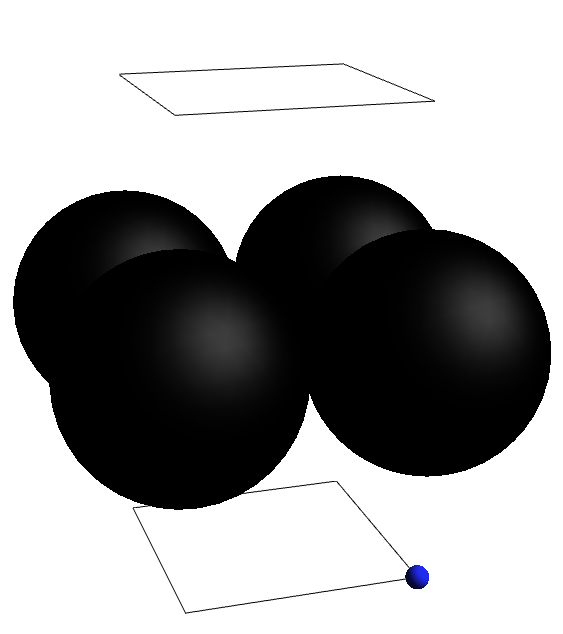
\includegraphics[width=0.6\linewidth]{figures/Kimcontraej}
	\caption{A black group with unconditional life.}
	\label{fig:Kimcontraejemplo}
\end{wrapfigure}\noindent Furthermore, if we omit the $9 \times 9 \times 9$ size restriction imposed by Kim, the phenomenon appears in its minimal expression on a $2 \times 2 \times 3$ board: a single horizontal layer $B_2$ at $z = 2$ separates the board into two distinct eyes $R_1$ and $R_3$, achieving unconditional life on its own, as illustrated in (Figure~\ref{fig:Kimcontraejemplo}) with the aid of the \href{https://github.com/10500awa/3dGo}{3dGo} tool.\footnote{Not only the sizes are arbitrary but the adjacencies are also arbitrary, according to the game nature. In both, his adjacency rule and the one present here, the counterexample works.}

\section{Behind the Curtain}\label{sec:behind_curtain}

Stepping back from the specific mechanics of captures, \textit{ko}, and life, this chapter has distilled the minimum mathematical structure required to represent Go. At the close of Part~I, we noted that constructing the game requires four elementary ingredients: \textit{where}, \textit{who}, \textit{what}, and \textit{how}. We now see that these four notions correspond directly to the components of the 3-tuple
\[
\Gamma = (G, E, \sim),
\]
where:
\begin{itemize}
	\item $G$ formalizes \textbf{where} the game takes place: the underlying set of playable positions.
	\item $E$ formalizes \textbf{who} participates: the set of states a position may assume, comprising the players together with a distinguished vacant state ($0 \in E$).
	\item $\sim \subseteq G \times G$ (equivalently, the adjacency relation $\sim$) formalizes \textbf{what} structures emerge on the board: the spatial relation between positions from which connections, groups, regions, territories, and liberties are derived.
\end{itemize}

And lastly, as we are in a game, $\Delta : \mathcal{T} \times \mathcal{J} \to \mathcal{T}$ formalizes \textbf{how}
the game evolves over time: the transition rule governing move legality, captures, and state progression.

In Part~III, we shall decouple and vary each of these components independently: first by altering the geometry of $(G, \sim)$ across dimensions and topologies, and subsequently by modifying $\Delta$ and the winning criteria. In doing so, we will not only generalize Go, but also show that a broad family of surrounding and connection games can be naturally unified within this same axiomatic framework.
\newpage